\documentclass[11pt]{article}

\usepackage[a4paper,margin=1in]{geometry}
\usepackage[T1]{fontenc}
\usepackage[utf8]{inputenc}
\usepackage{amsmath}
\usepackage{graphicx}
\usepackage{booktabs}
\usepackage{tabularx}
\usepackage{array}
\usepackage{subcaption}
\usepackage{float}
\usepackage{hyperref}
\usepackage{enumitem}

\hypersetup{
    colorlinks=true,
    linkcolor=blue,
    citecolor=blue,
    urlcolor=blue
}

\graphicspath{{figures/interference/}}

\title{Finite-Blocklength Latency Minimization for Uplink and Downlink Communications:\\Method Results: Interference}
\author{}
\date{July 6, 2026}

\begin{document}

\maketitle

\begin{abstract}
This document collects the exported interference figures for uplink and
downlink under payload completion. Throughout, the \emph{Training Only Method}
is used as the benchmark for the \emph{Training + Testing Method}. The uplink
figures mostly show moderate interference reshaping inside a similar operating
regime. The downlink figures are more structural, especially when users are
removed from the active set and their traces drop toward \(-300\) dB.
\end{abstract}

\section{Scope and Naming}

This document is intentionally interference-only. The terminology is aligned
with the companion theory report:
\begin{itemize}[leftmargin=1.5em]
    \item \textbf{Training Only Method}: direct online optimization during scheduling,
    \item \textbf{Training + Testing Method}: a separate training stage followed by testing-stage inference,
    \item \textbf{Payload completion}: the scenario where each user continues until its remaining payload is exhausted.
\end{itemize}

\section{Uplink Payload Completion}

The uplink payload-completion interference picture stays fairly close across the
two methods. The benchmark does improve final SINR for users 1 and 2, but the
overall difference remains moderate rather than dramatic.

\begin{table}[H]
\centering
\small
\caption{Uplink payload-completion per-user SINR summary}
\renewcommand{\arraystretch}{1.15}
\begin{tabularx}{\textwidth}{>{\centering\arraybackslash}p{0.10\textwidth} >{\centering\arraybackslash}p{0.18\textwidth} >{\centering\arraybackslash}p{0.18\textwidth} X}
\toprule
User & Training Only init/final & Training + Testing init/final & Reading \\
\midrule
0 & \(-3.359/-3.396\) dB & \(-3.359/-2.908\) dB & Training + Testing is better on this user, but not enough to change the system outcome. \\
1 & \(-4.649/-4.006\) dB & \(-4.649/-4.592\) dB & Benchmark has the clearest SINR gain here. \\
2 & \(-2.173/-2.459\) dB & \(-2.173/-2.743\) dB & Benchmark ends less negative. \\
\bottomrule
\end{tabularx}
\end{table}

\begin{figure}[H]
\centering
\begin{subfigure}[t]{0.48\textwidth}
    \centering
    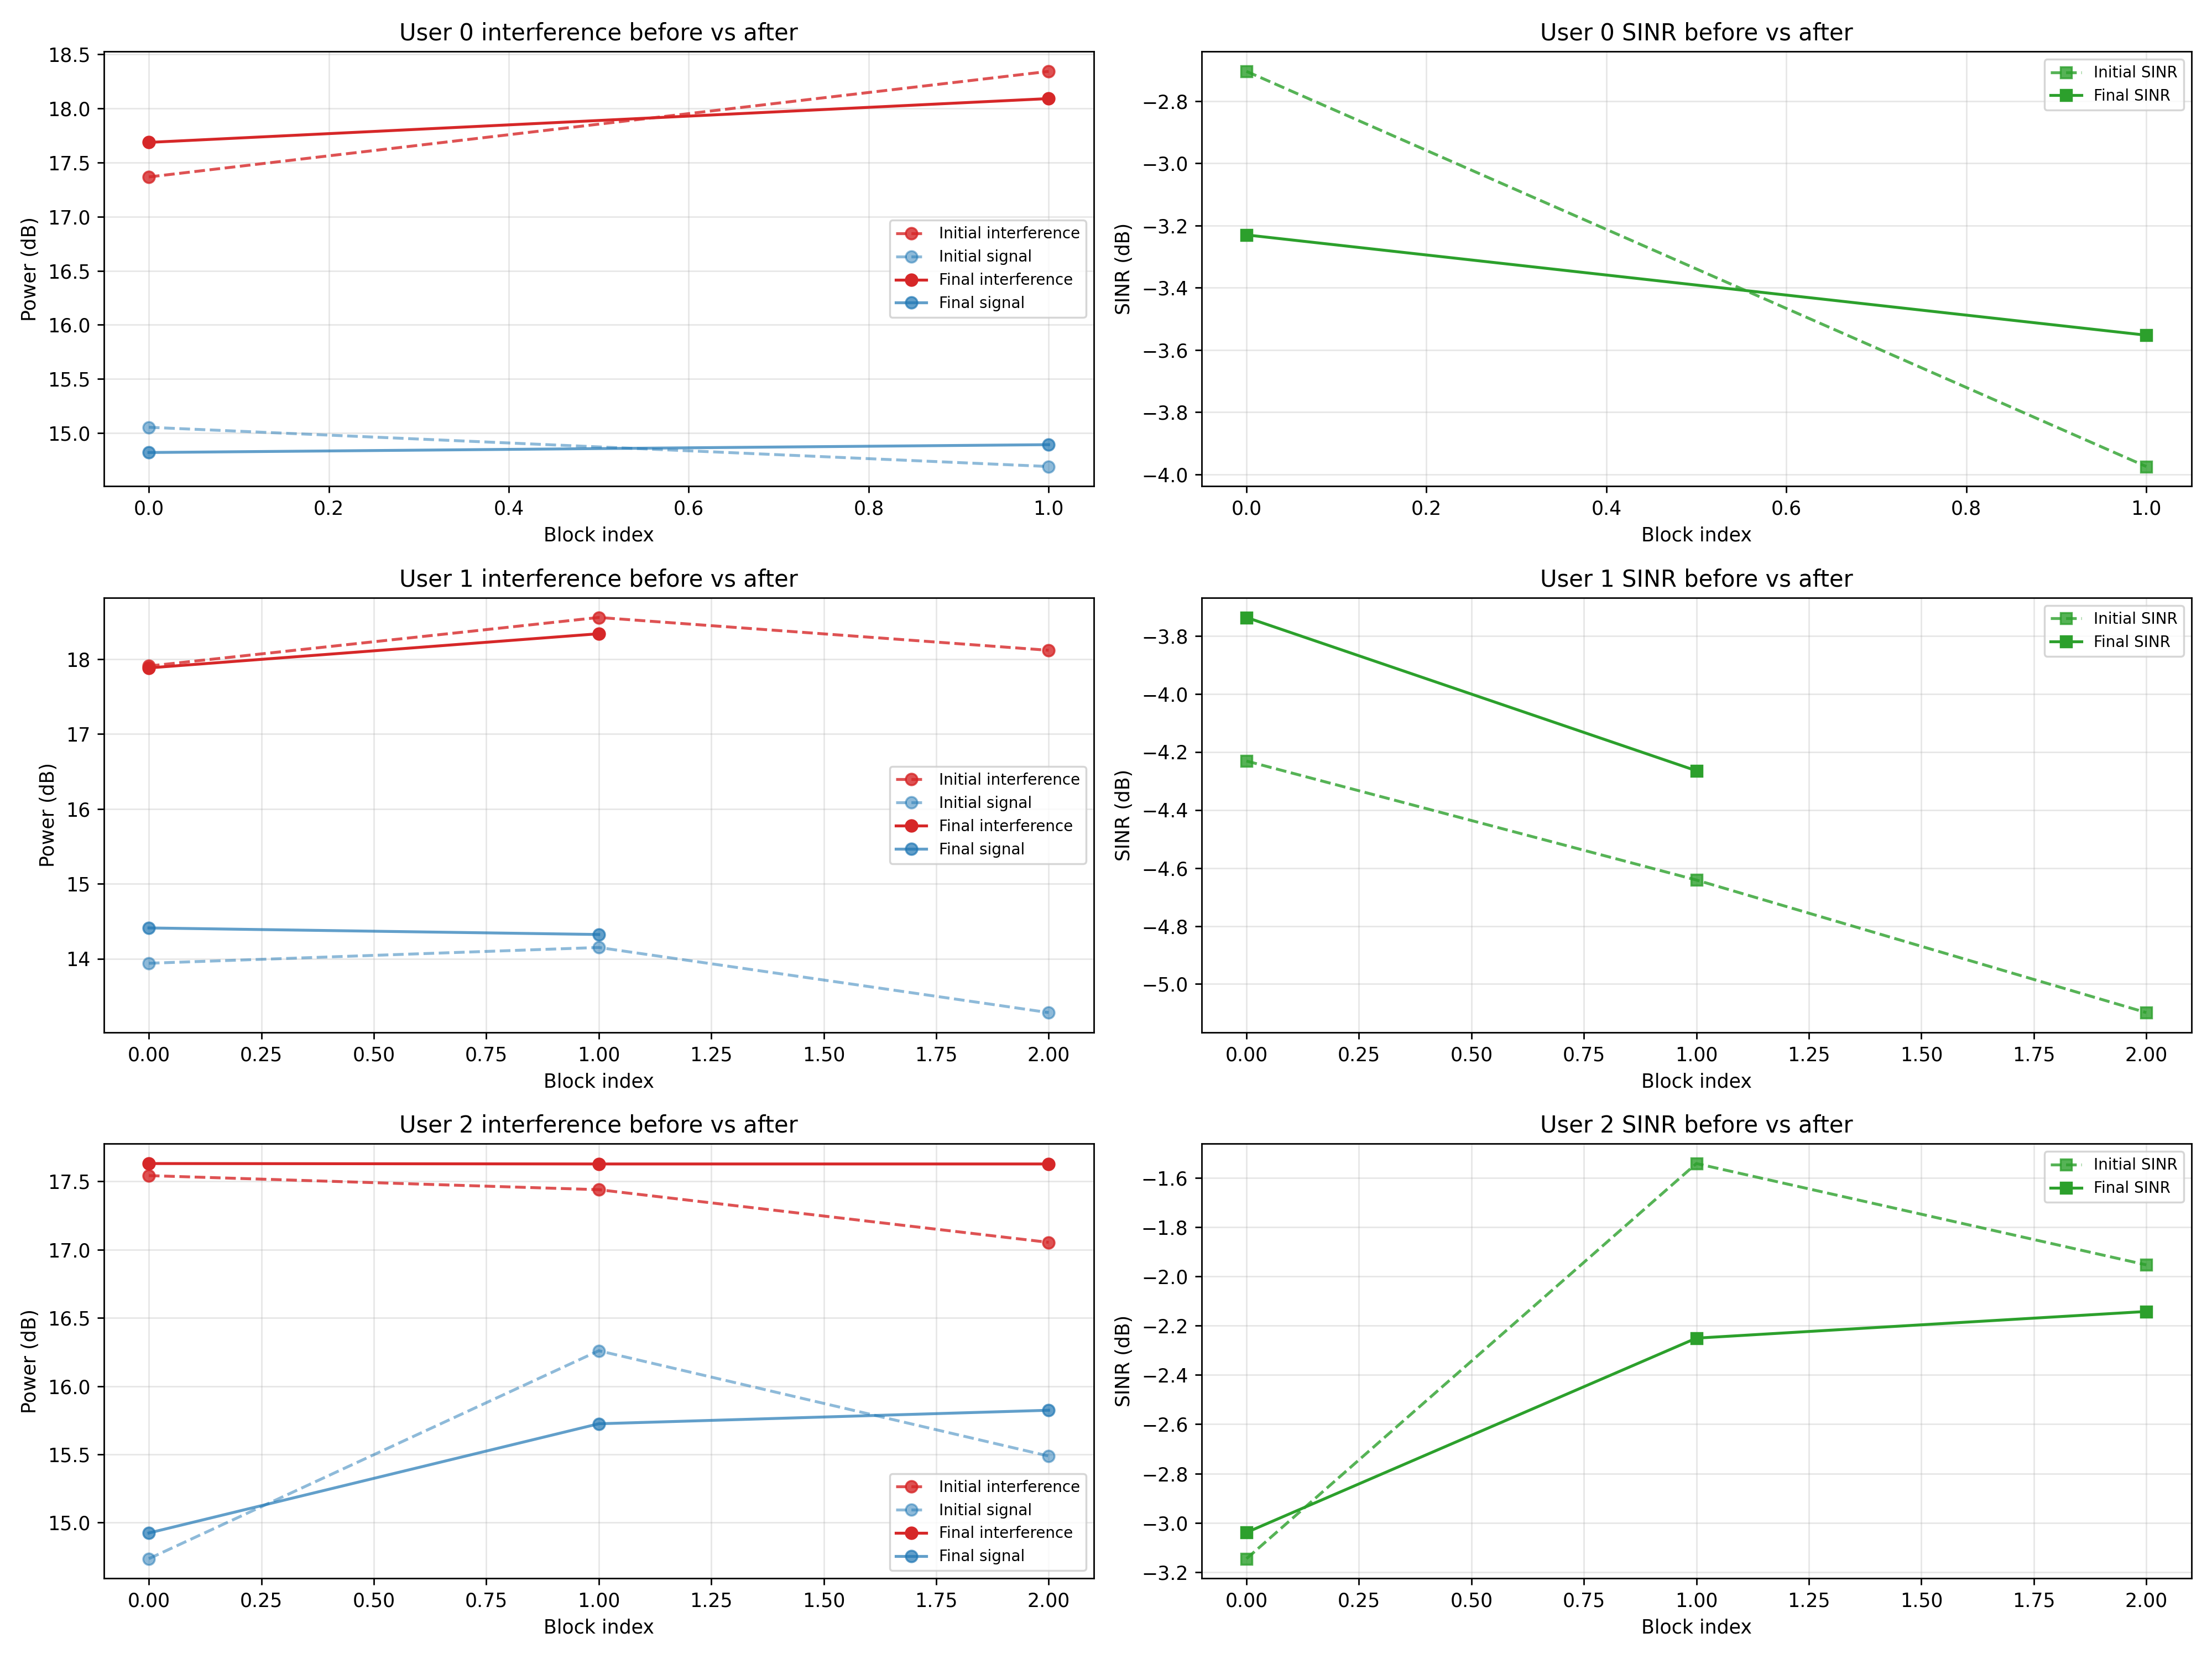
\includegraphics[width=\textwidth]{ul_payload_training_only__per_user_interference_before_after.png}
    \caption{Training Only Method}
\end{subfigure}
\hfill
\begin{subfigure}[t]{0.48\textwidth}
    \centering
    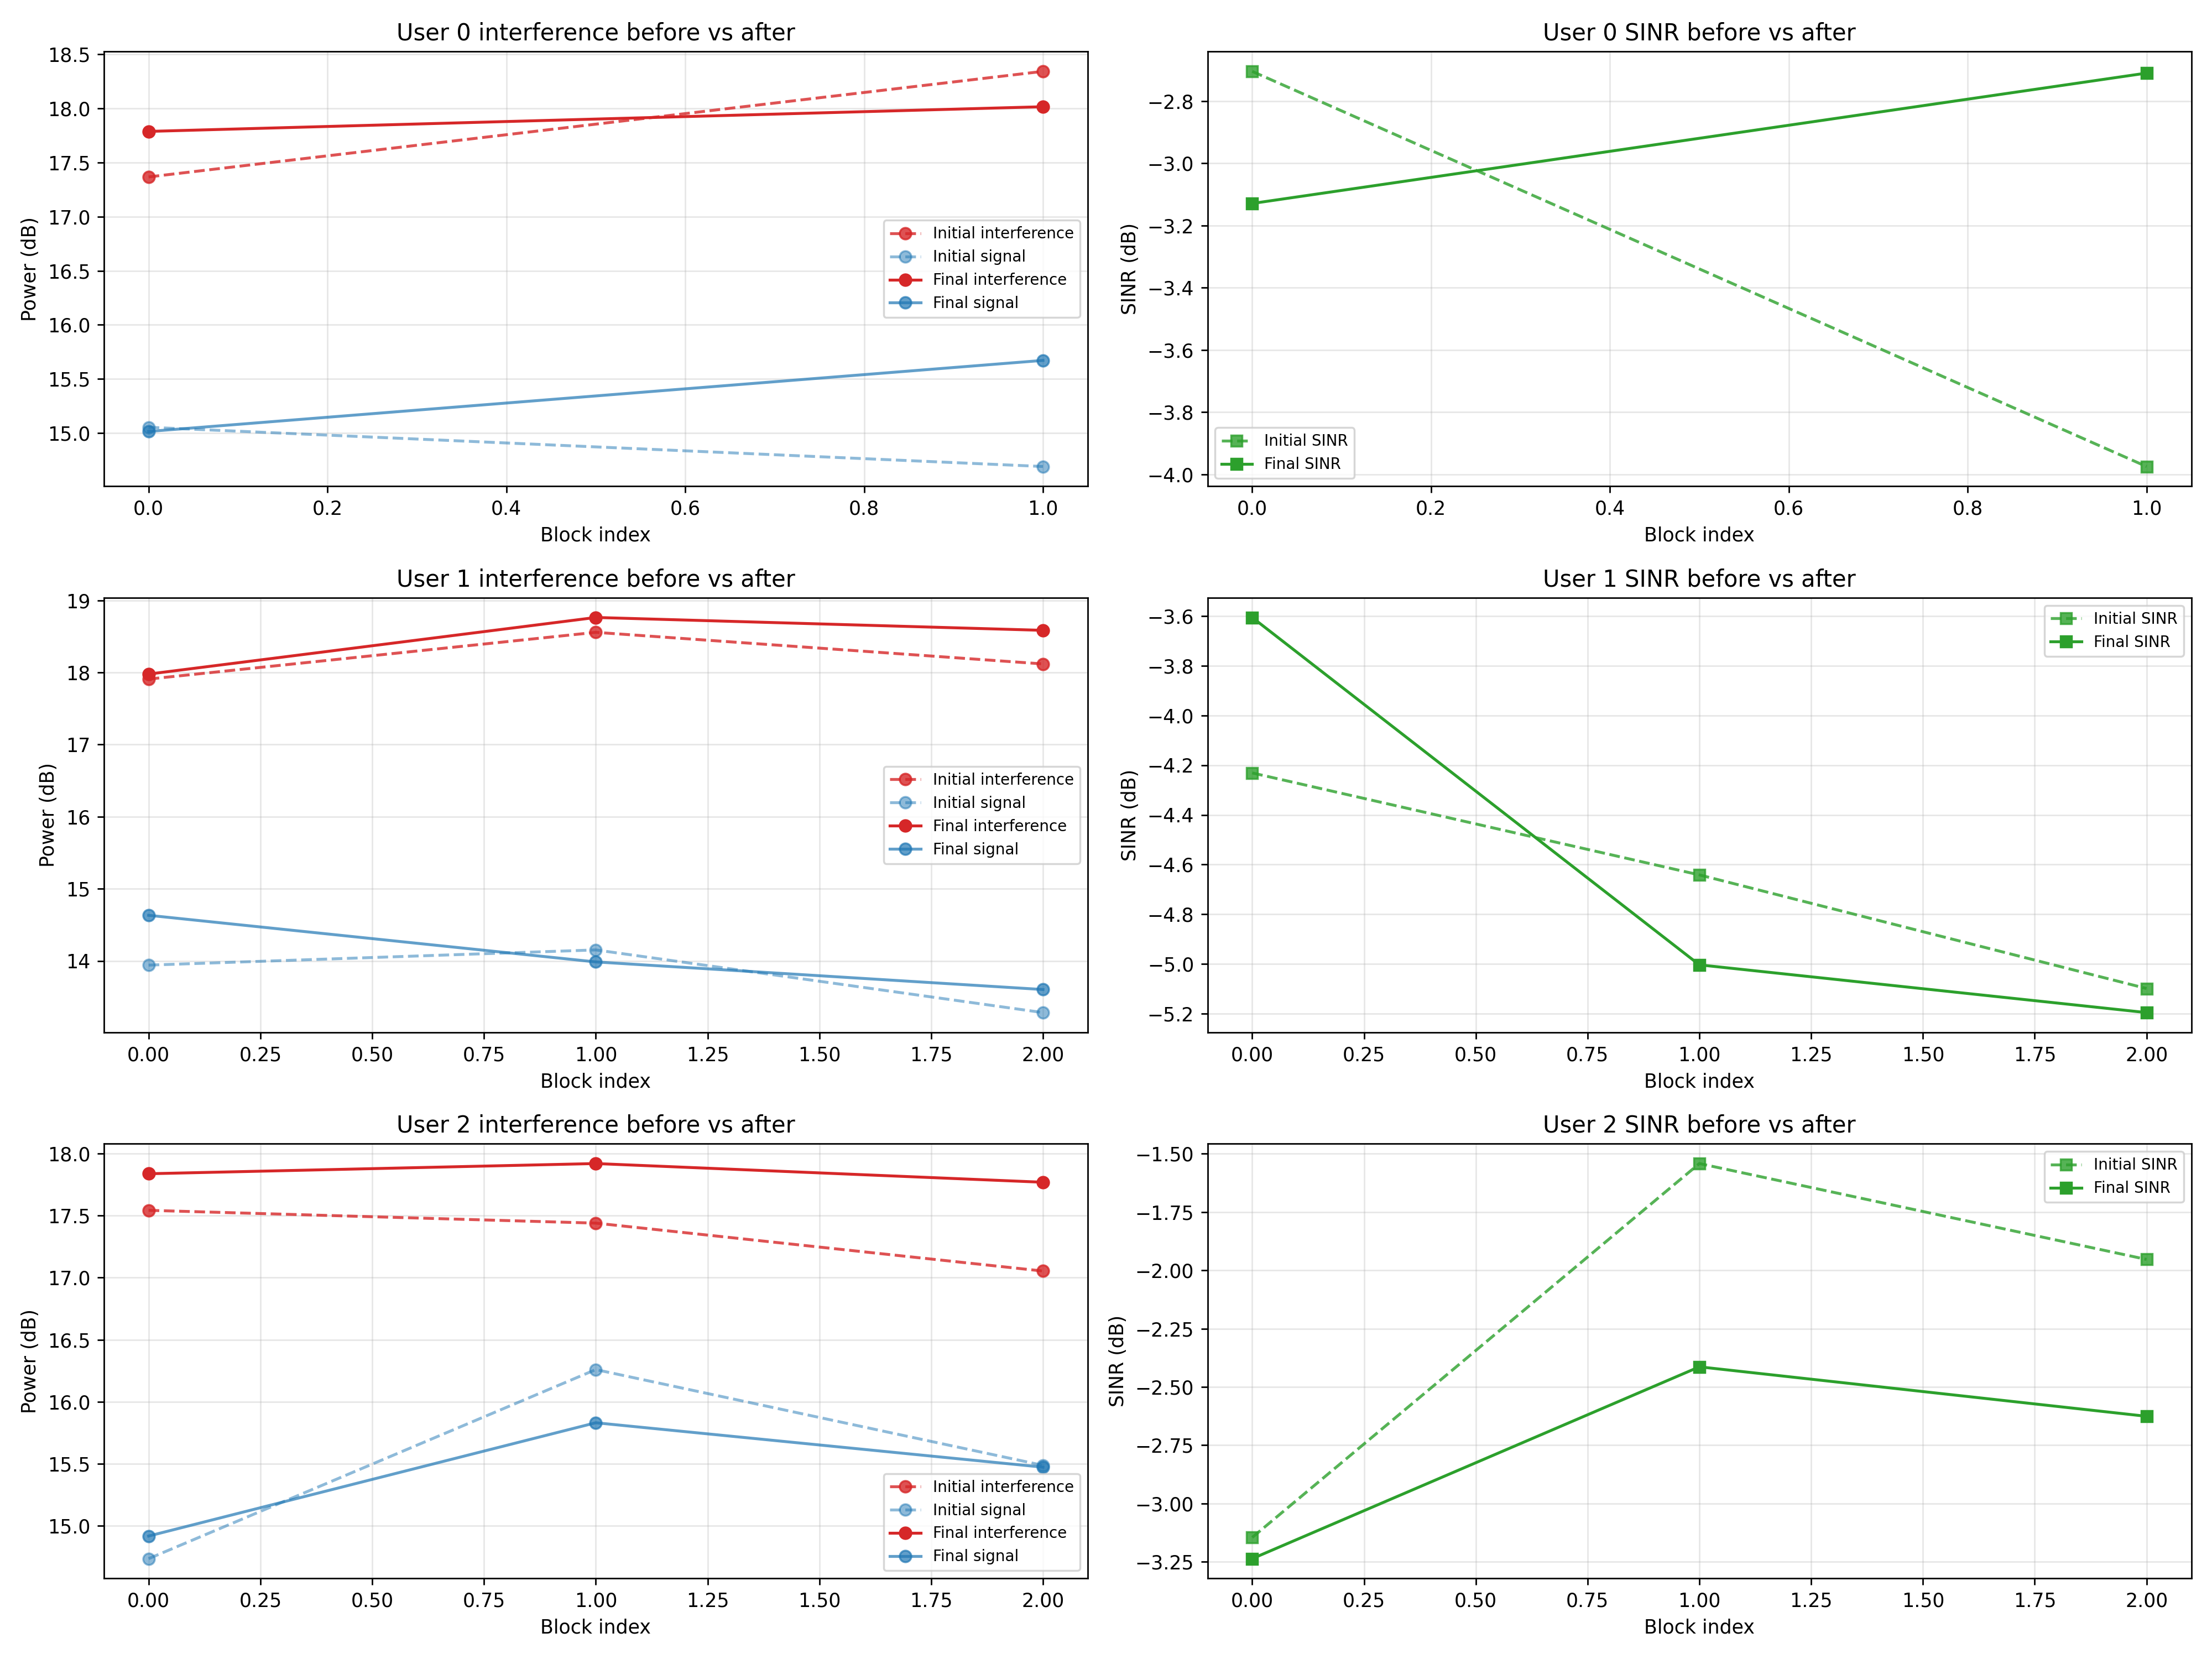
\includegraphics[width=\textwidth]{ul_payload_training_testing__per_user_interference_before_after.png}
    \caption{Training + Testing Method}
\end{subfigure}
\caption{Uplink payload-completion per-user interference before/after comparison.}
\end{figure}

\begin{figure}[H]
\centering
\begin{subfigure}[t]{0.48\textwidth}
    \centering
    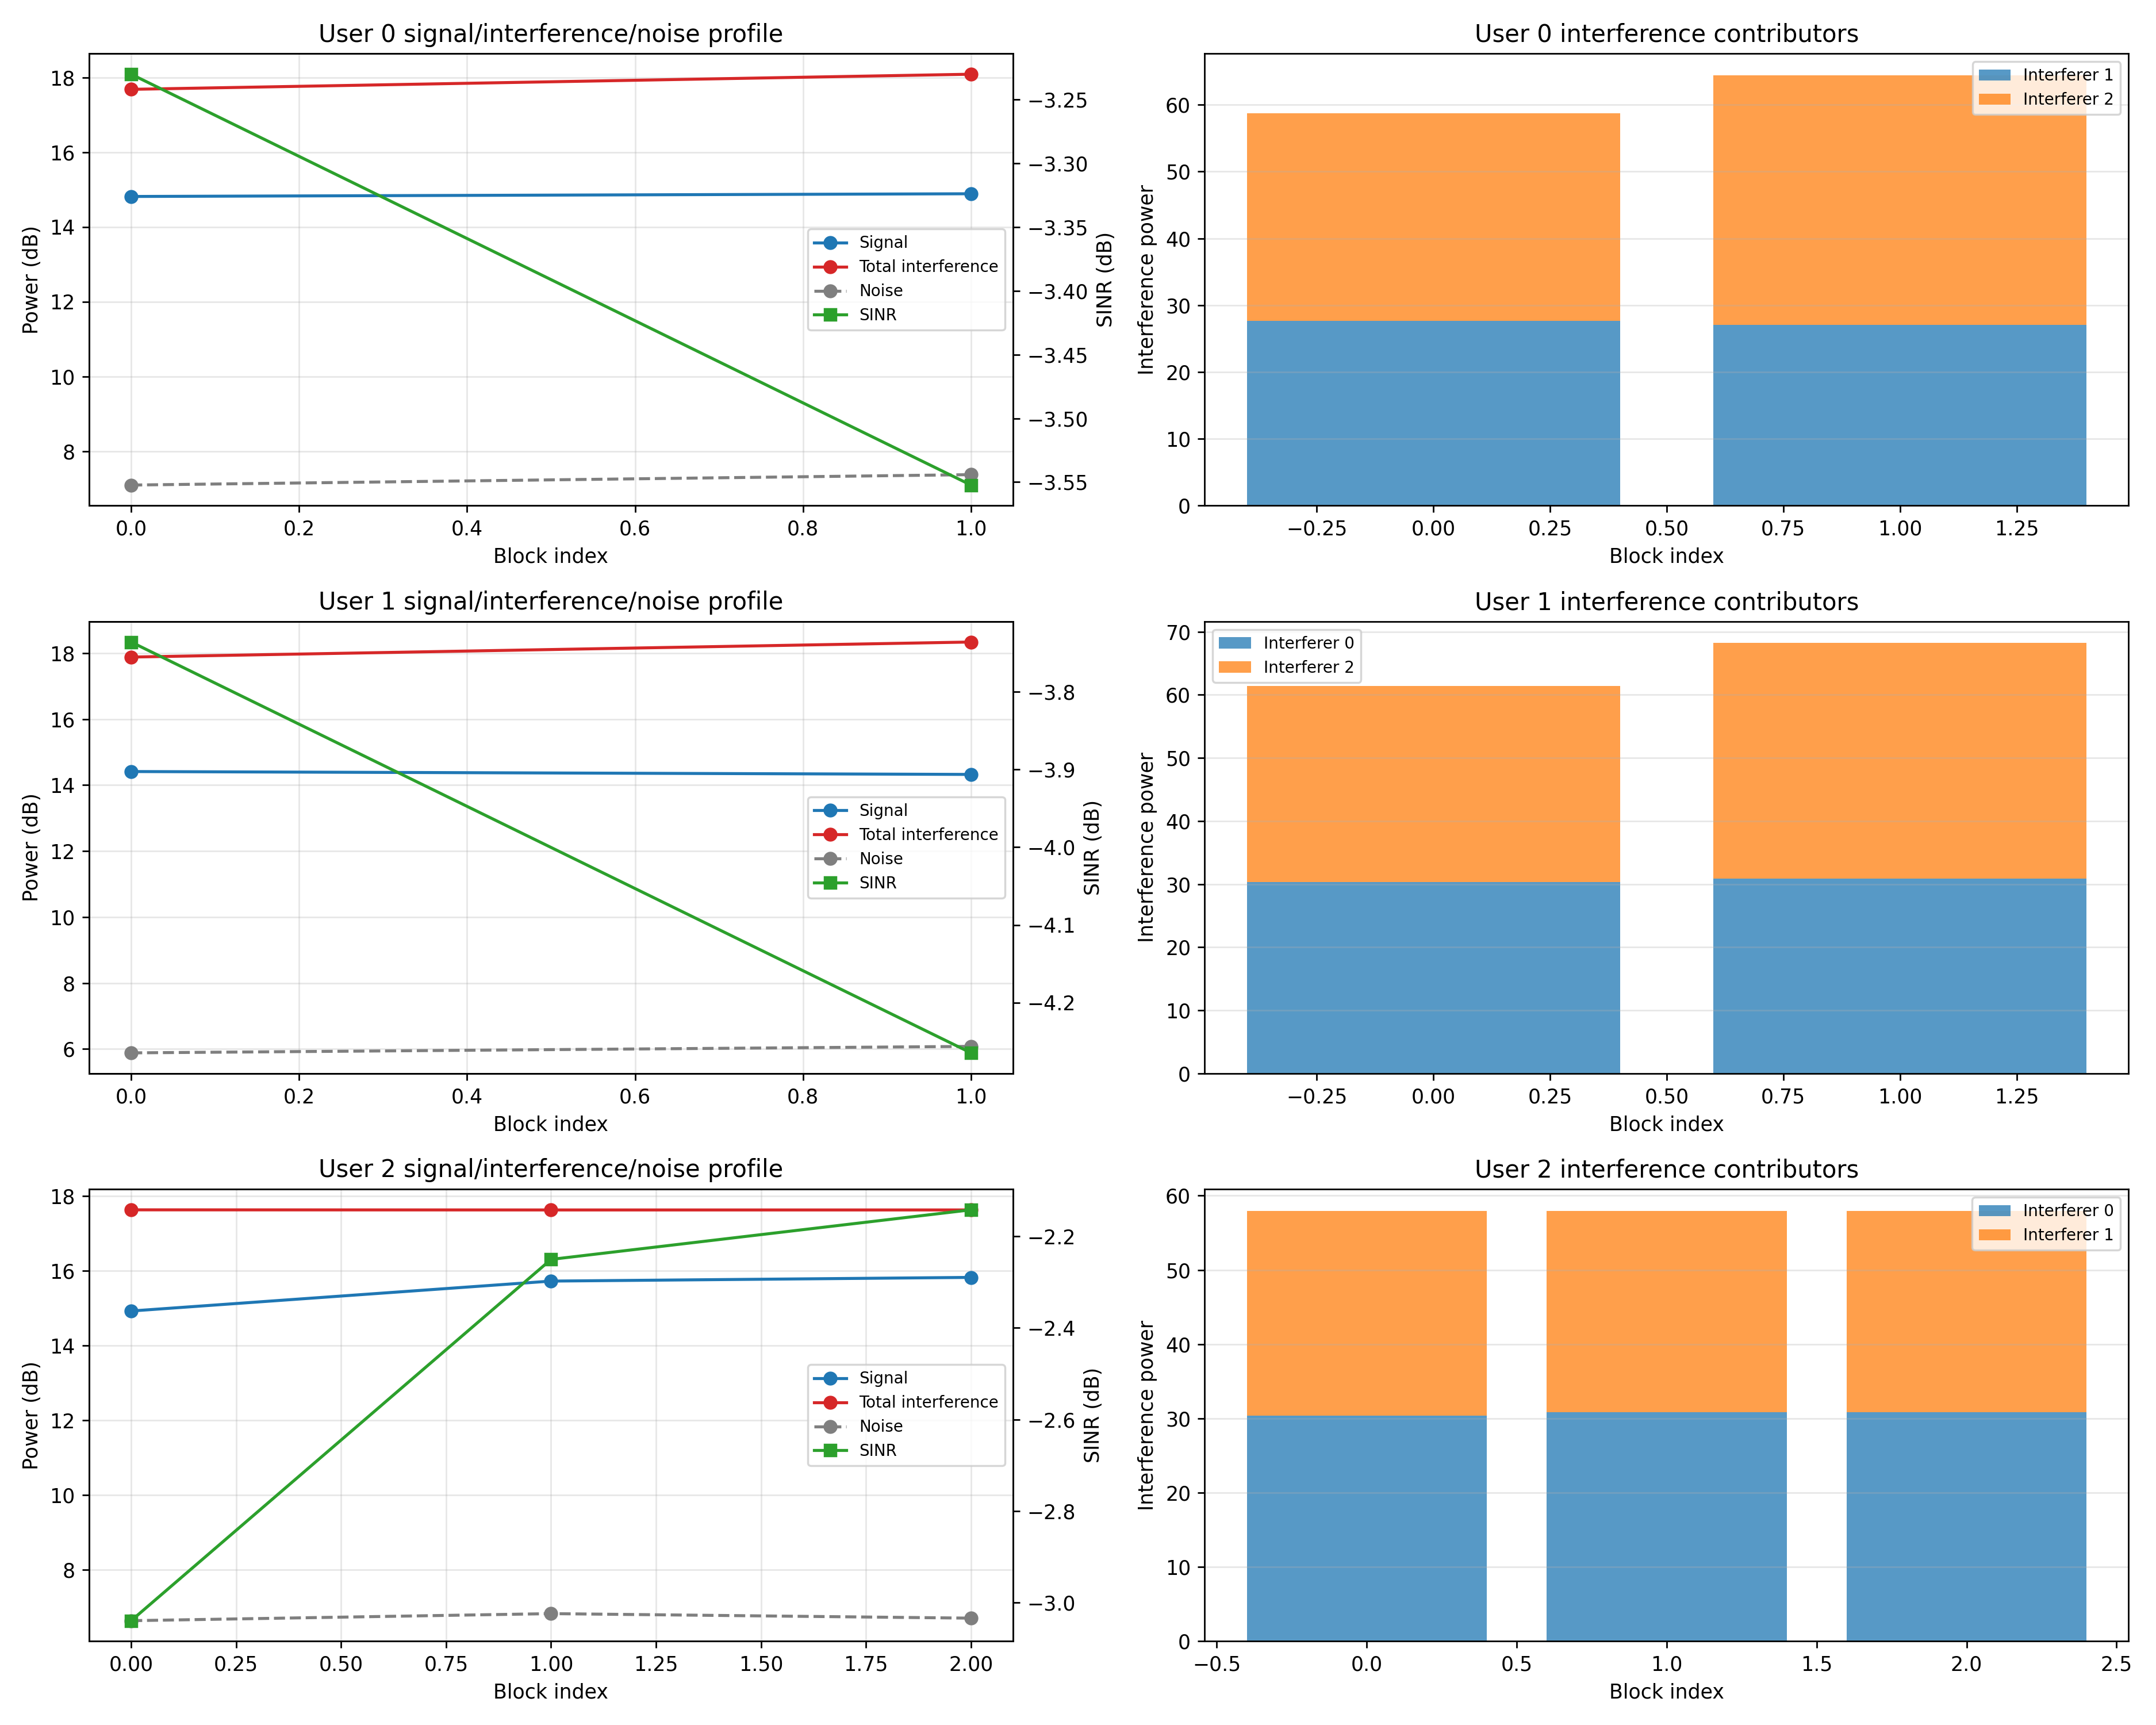
\includegraphics[width=\textwidth]{ul_payload_training_only__per_user_interference_profiles.png}
    \caption{Training Only Method}
\end{subfigure}
\hfill
\begin{subfigure}[t]{0.48\textwidth}
    \centering
    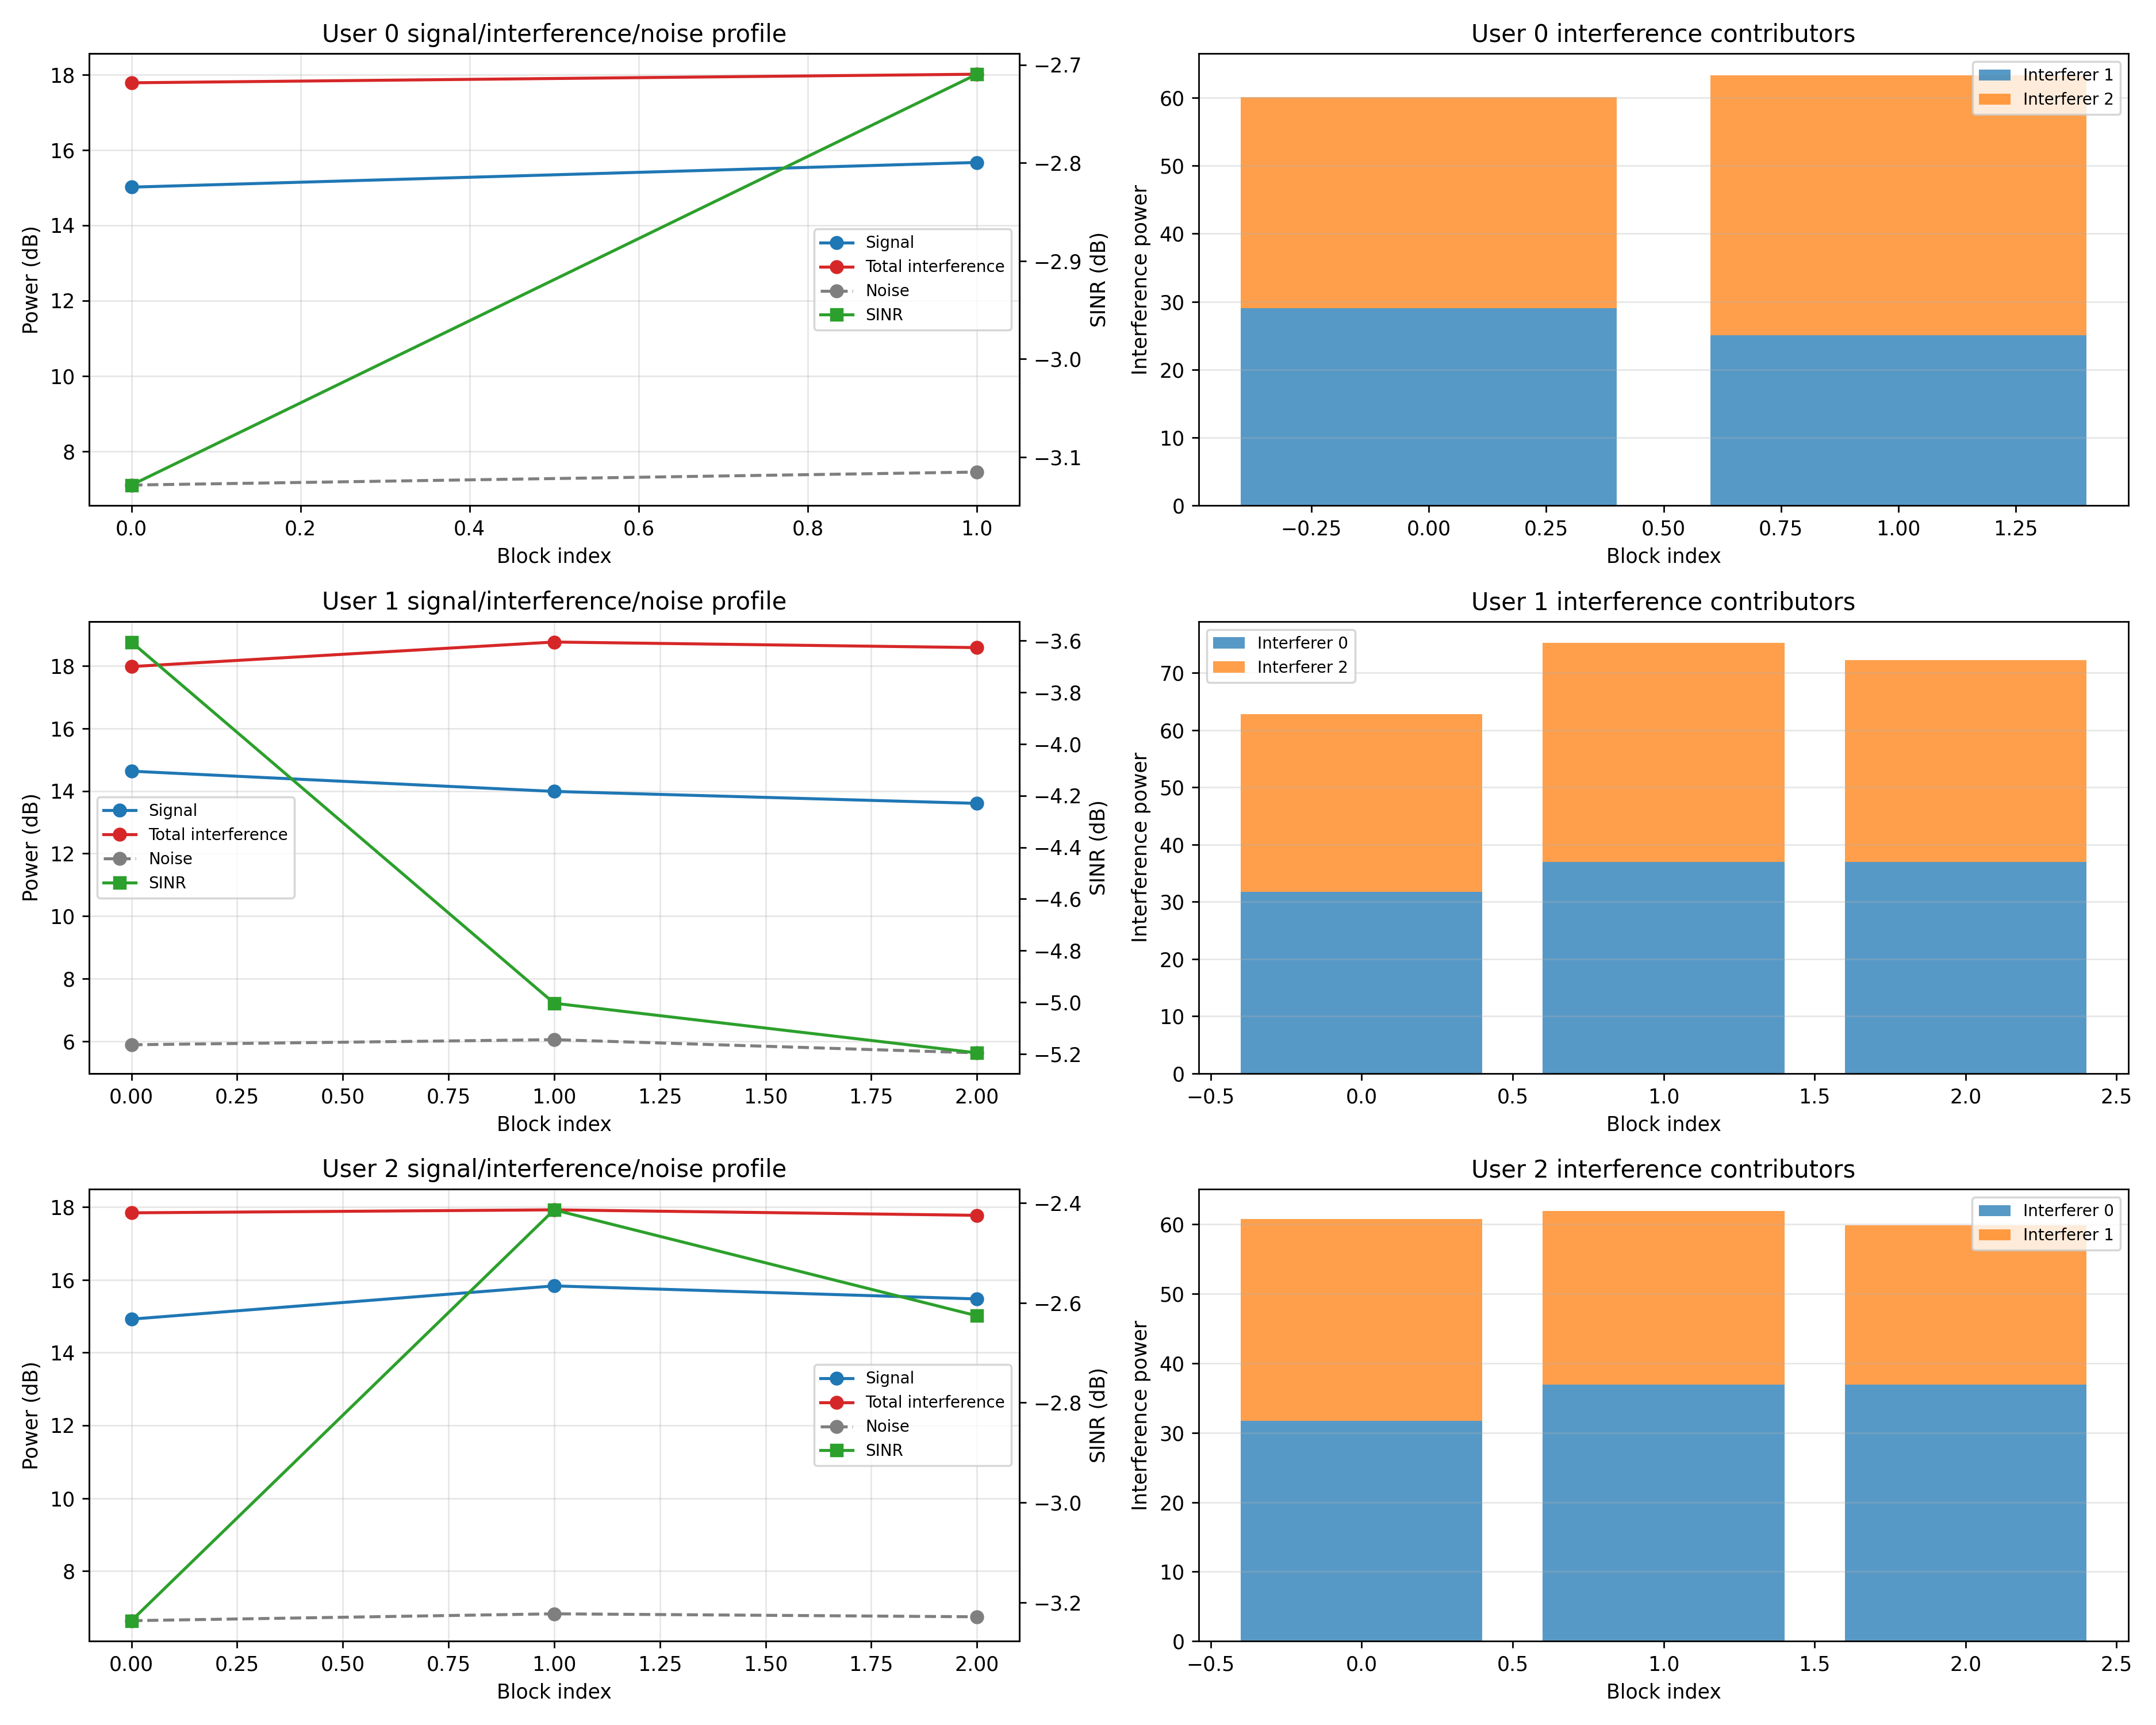
\includegraphics[width=\textwidth]{ul_payload_training_testing__per_user_interference_profiles.png}
    \caption{Training + Testing Method}
\end{subfigure}
\caption{Uplink payload-completion per-user interference profiles.}
\end{figure}

\begin{figure}[H]
\centering
\begin{subfigure}[t]{0.48\textwidth}
    \centering
    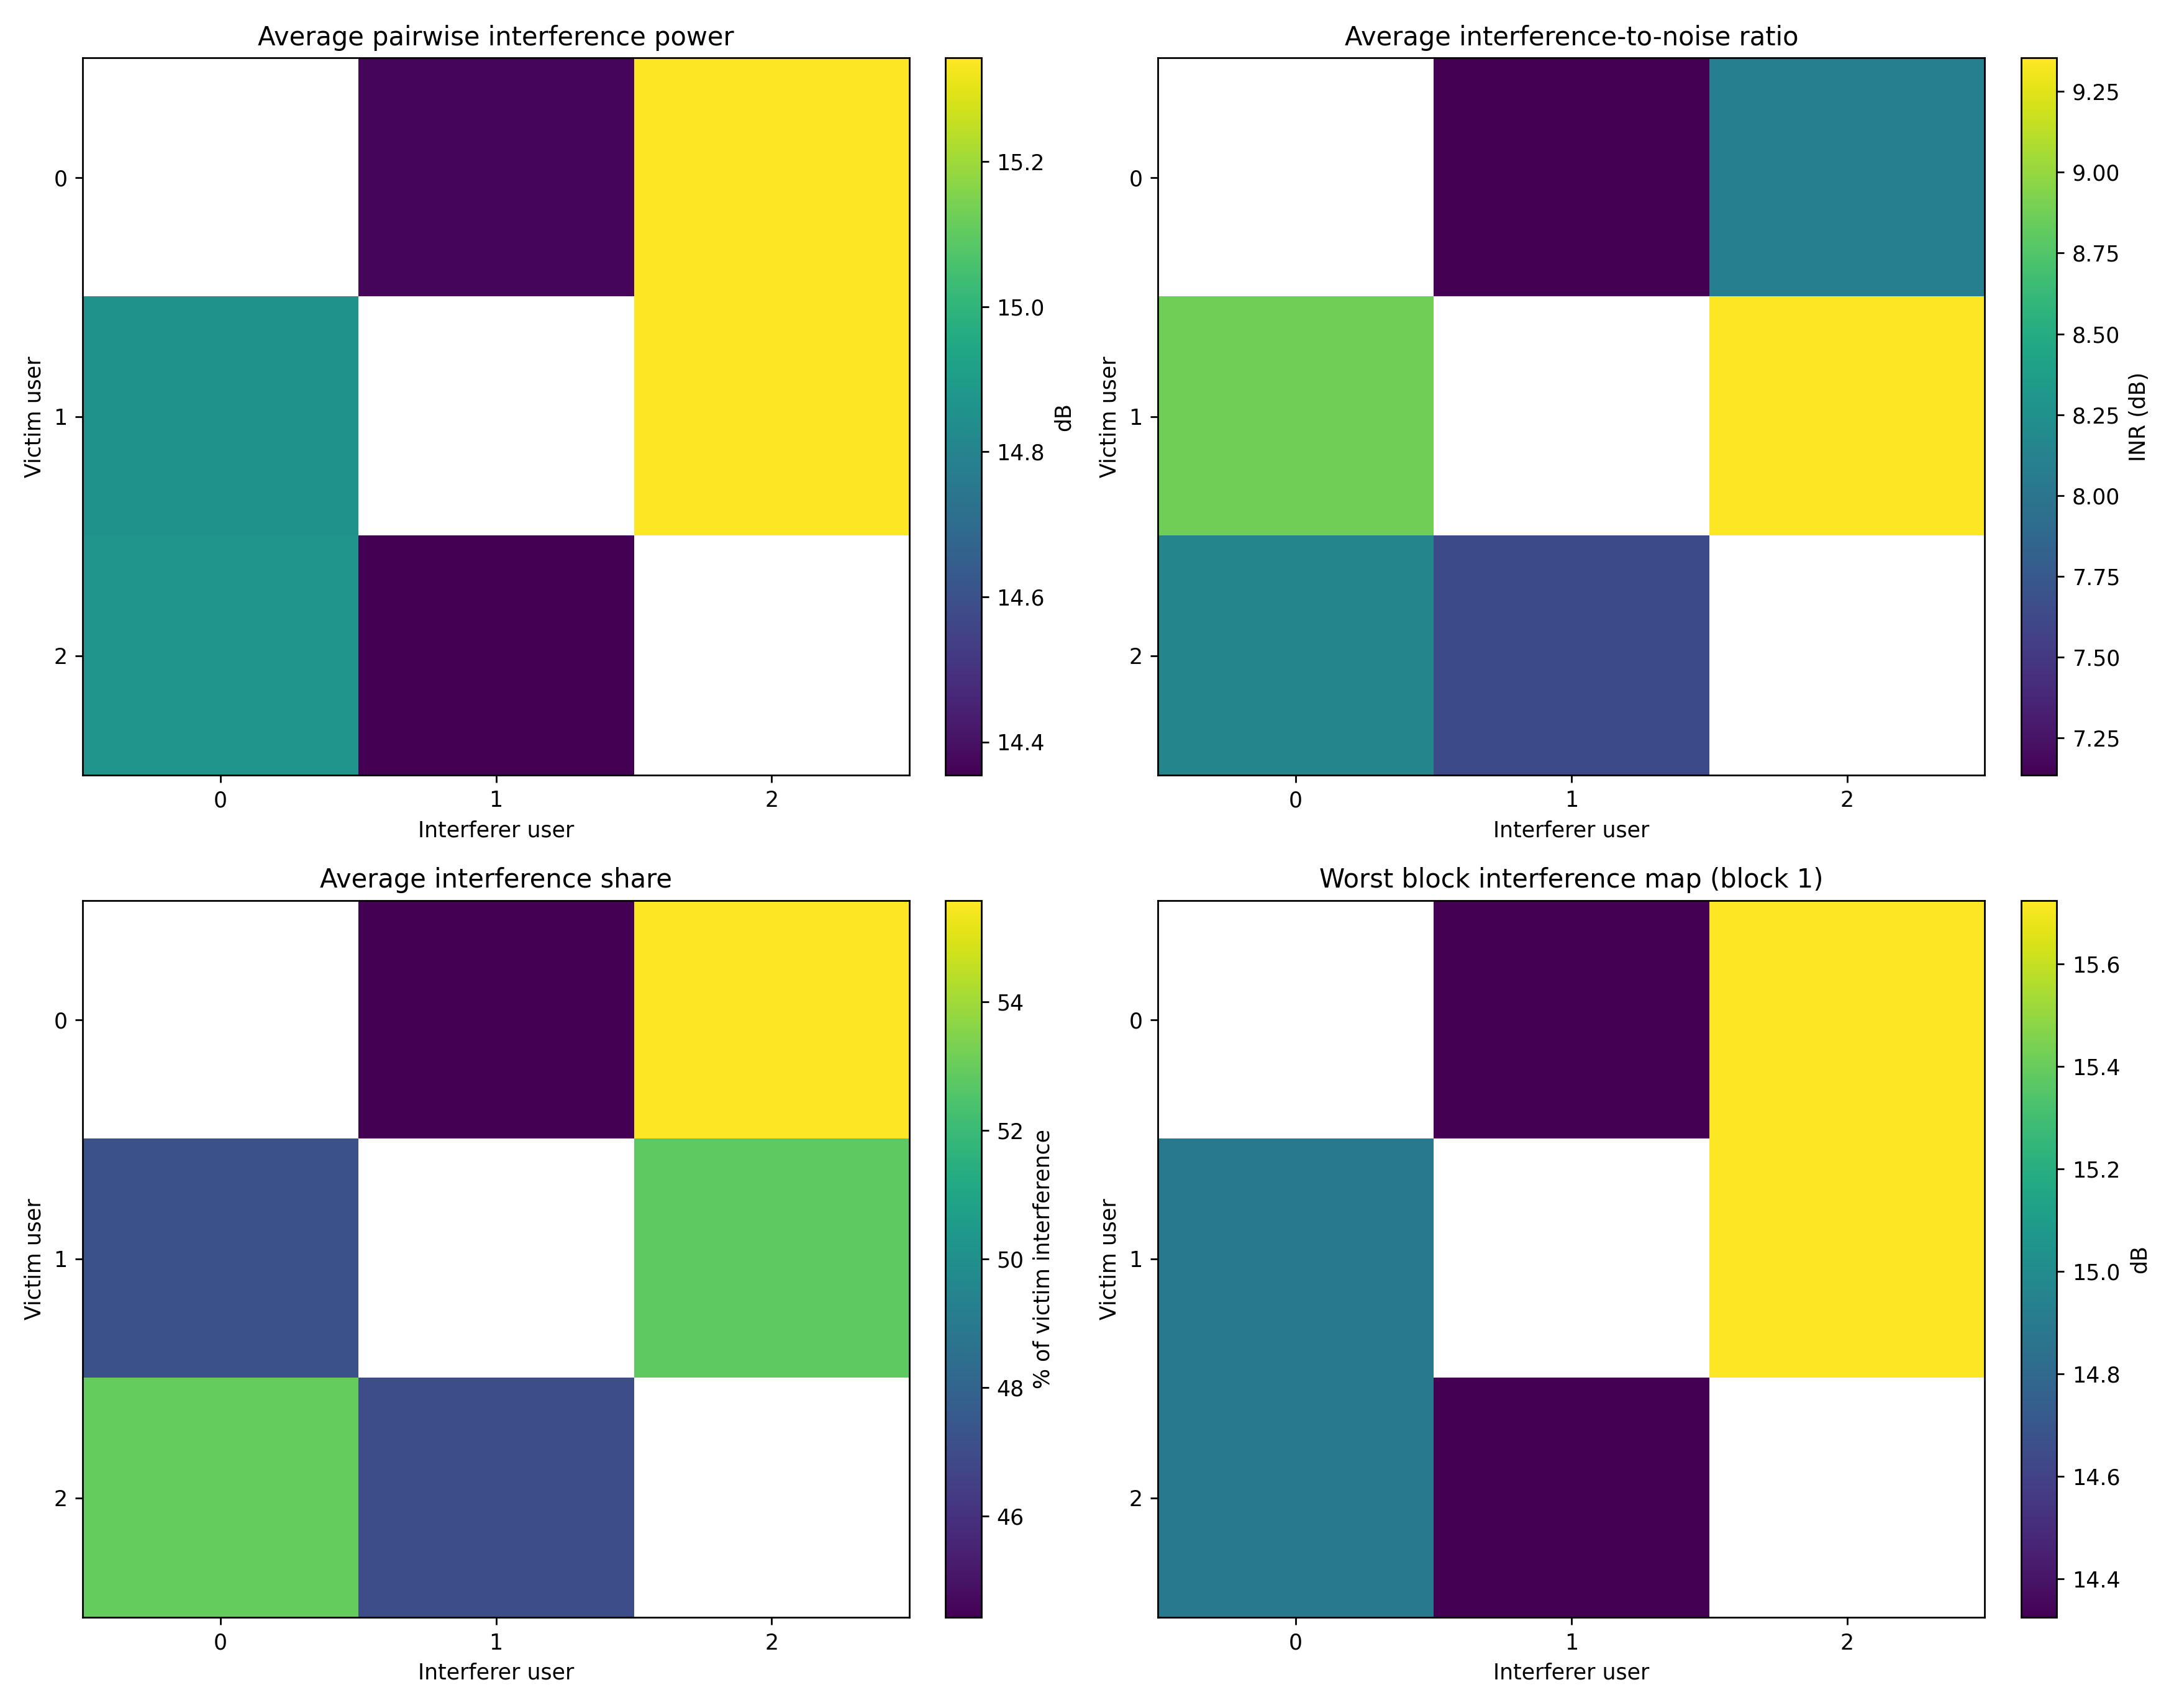
\includegraphics[width=\textwidth]{ul_payload_training_only__interference_heatmaps.png}
    \caption{Training Only Method}
\end{subfigure}
\hfill
\begin{subfigure}[t]{0.48\textwidth}
    \centering
    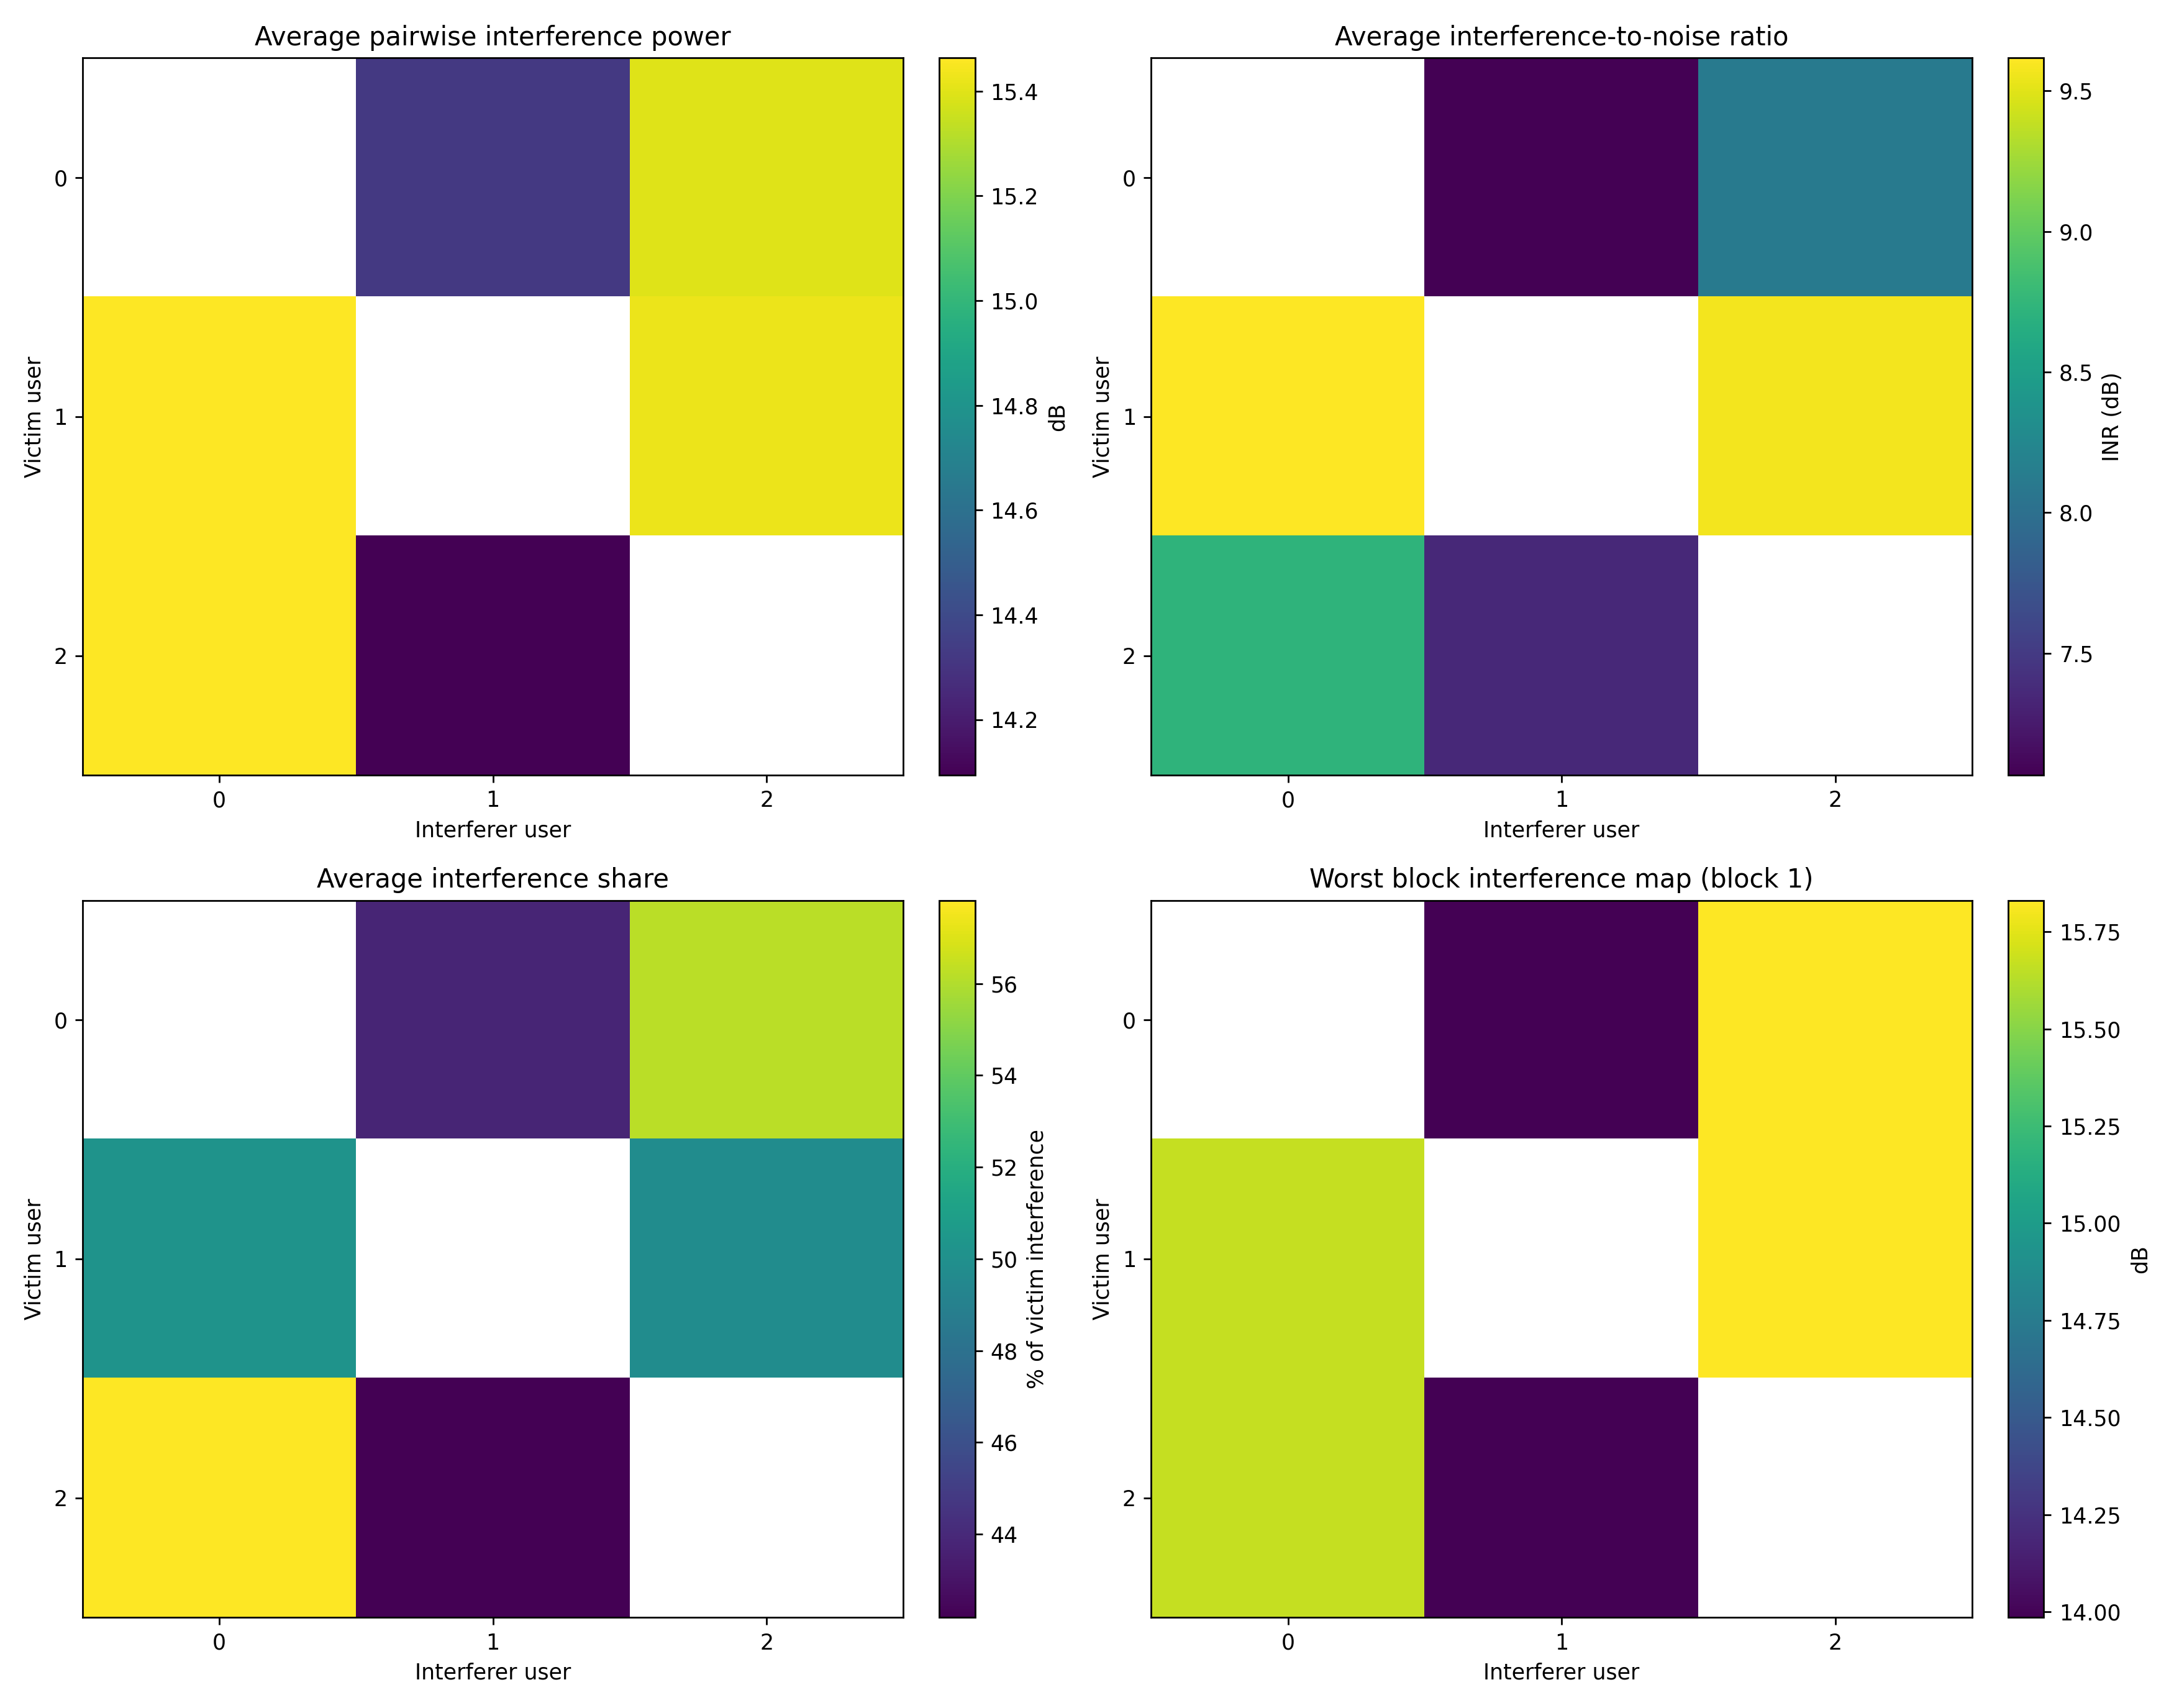
\includegraphics[width=\textwidth]{ul_payload_training_testing__interference_heatmaps.png}
    \caption{Training + Testing Method}
\end{subfigure}
\caption{Uplink payload-completion interference heatmaps.}
\end{figure}

\begin{figure}[H]
\centering
\begin{subfigure}[t]{0.48\textwidth}
    \centering
    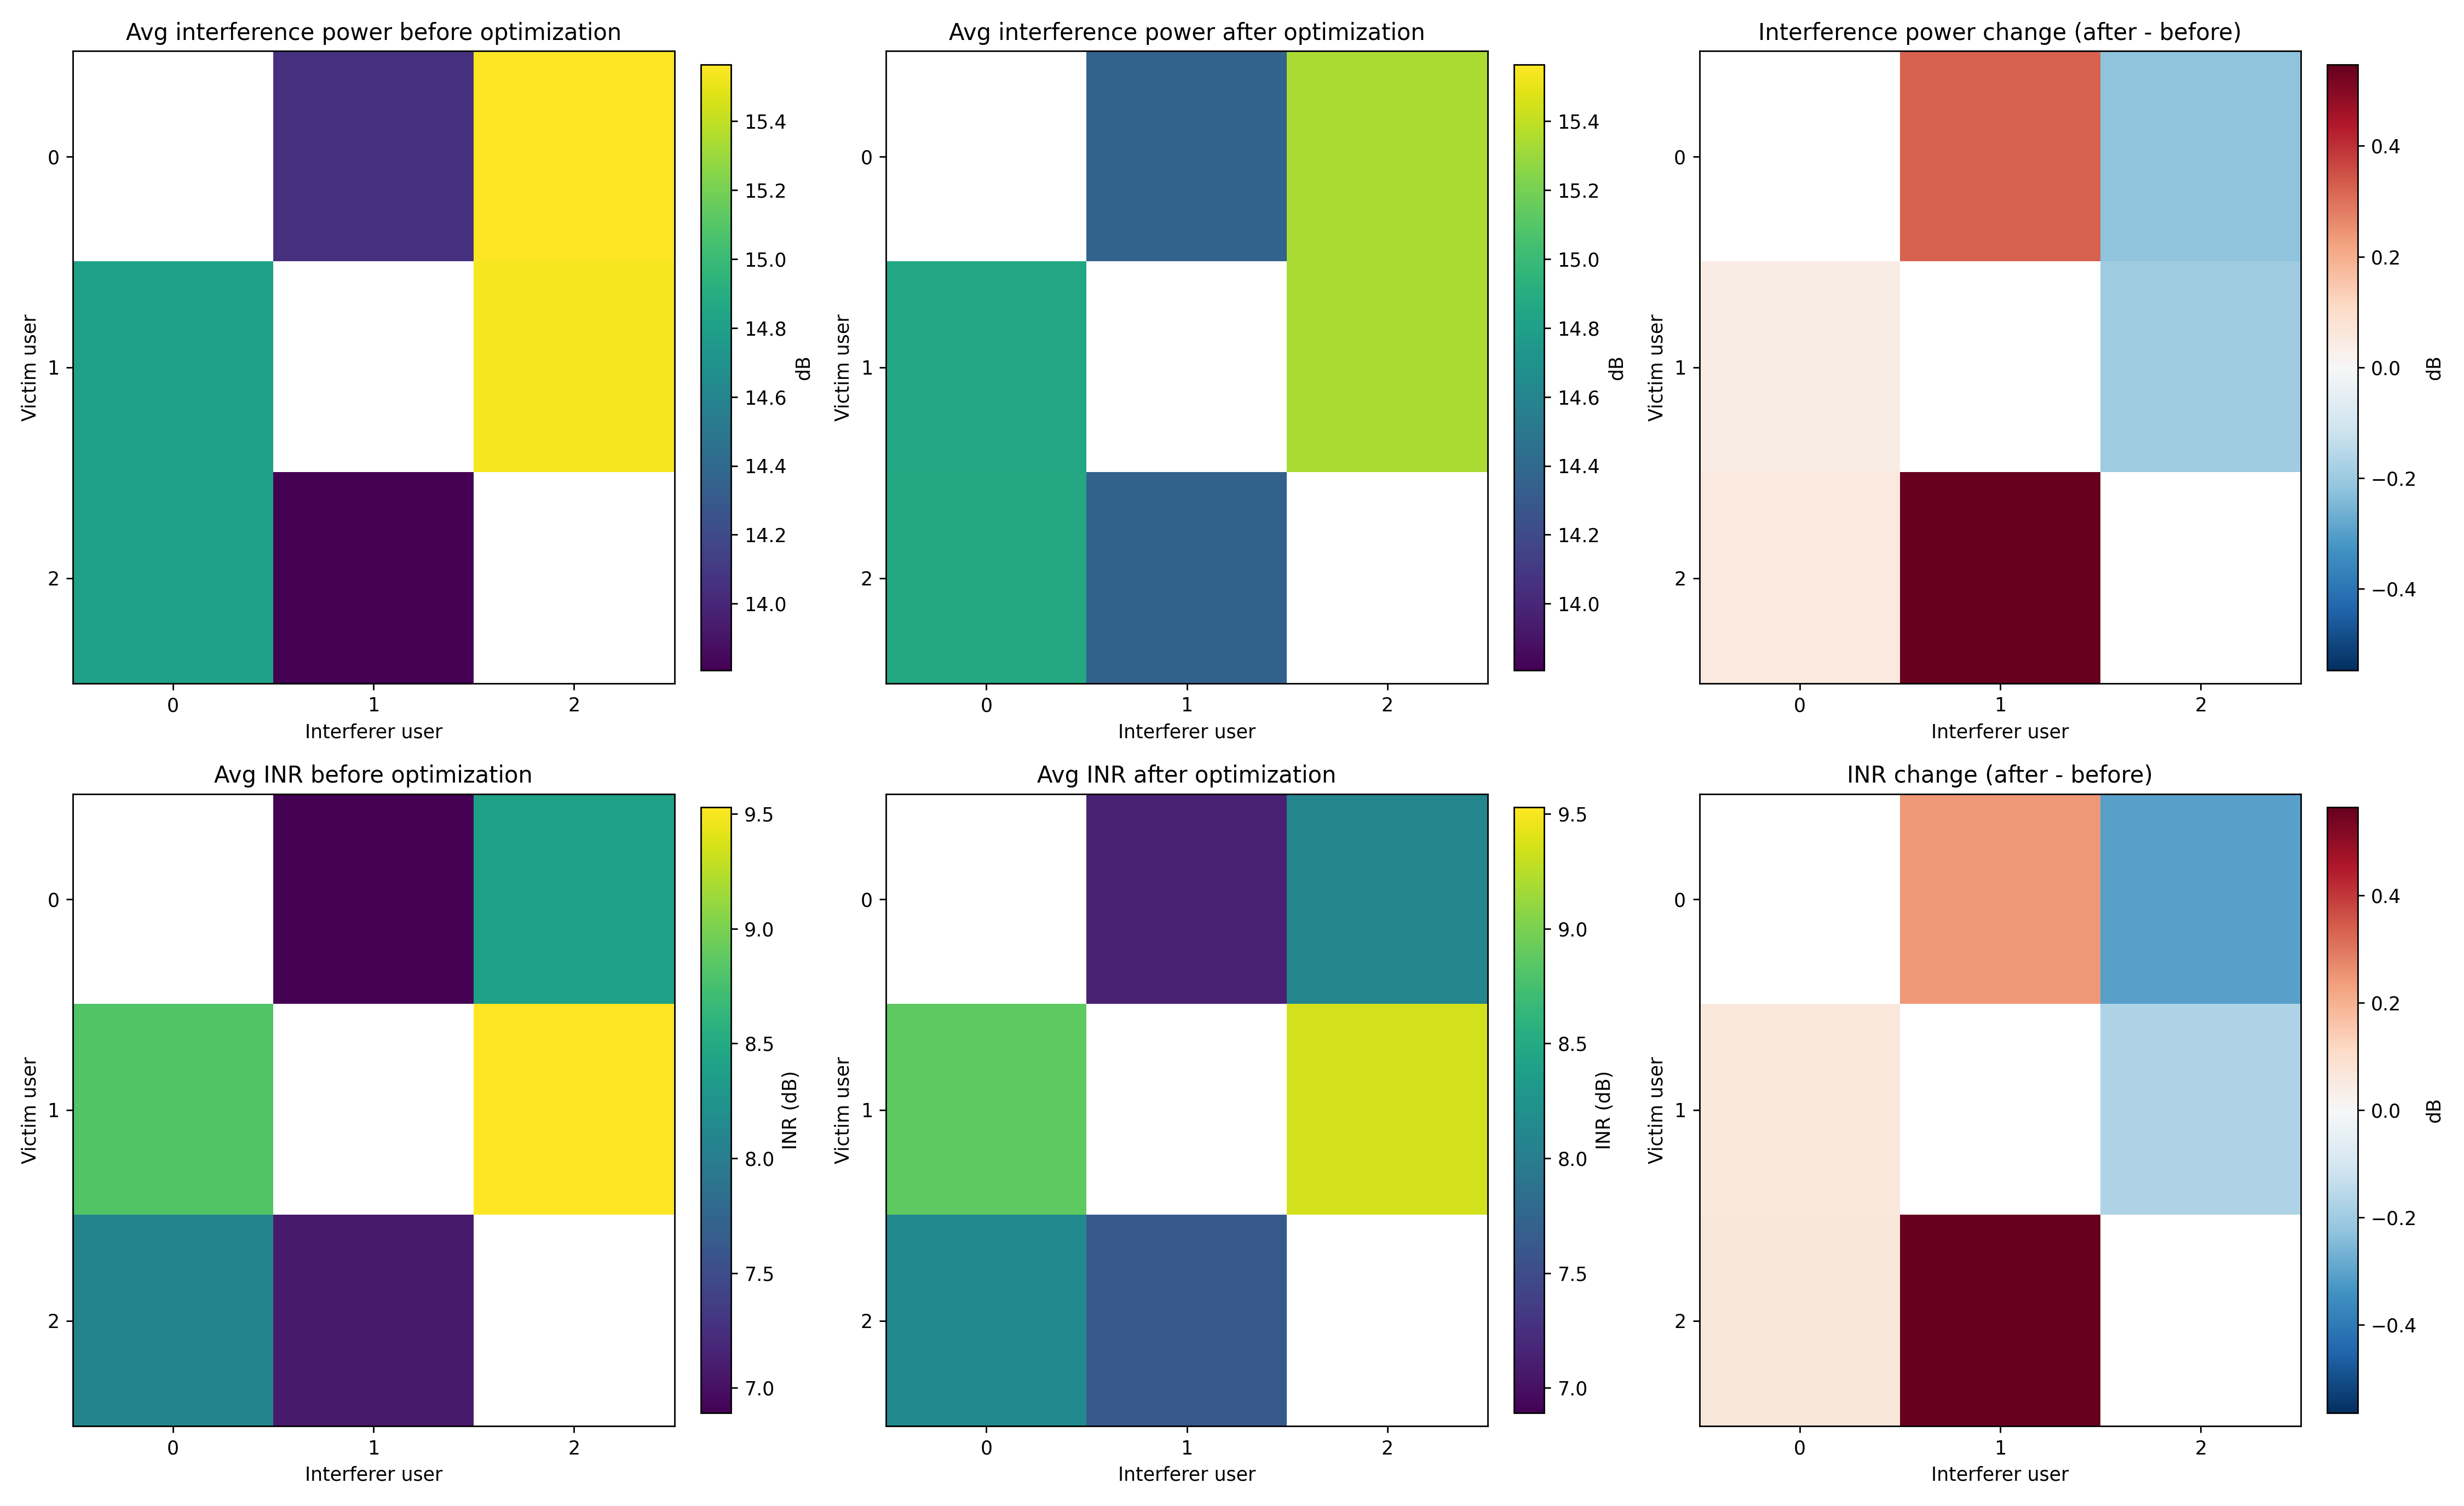
\includegraphics[width=\textwidth]{ul_payload_training_only__interference_before_after_heatmaps.png}
    \caption{Training Only Method}
\end{subfigure}
\hfill
\begin{subfigure}[t]{0.48\textwidth}
    \centering
    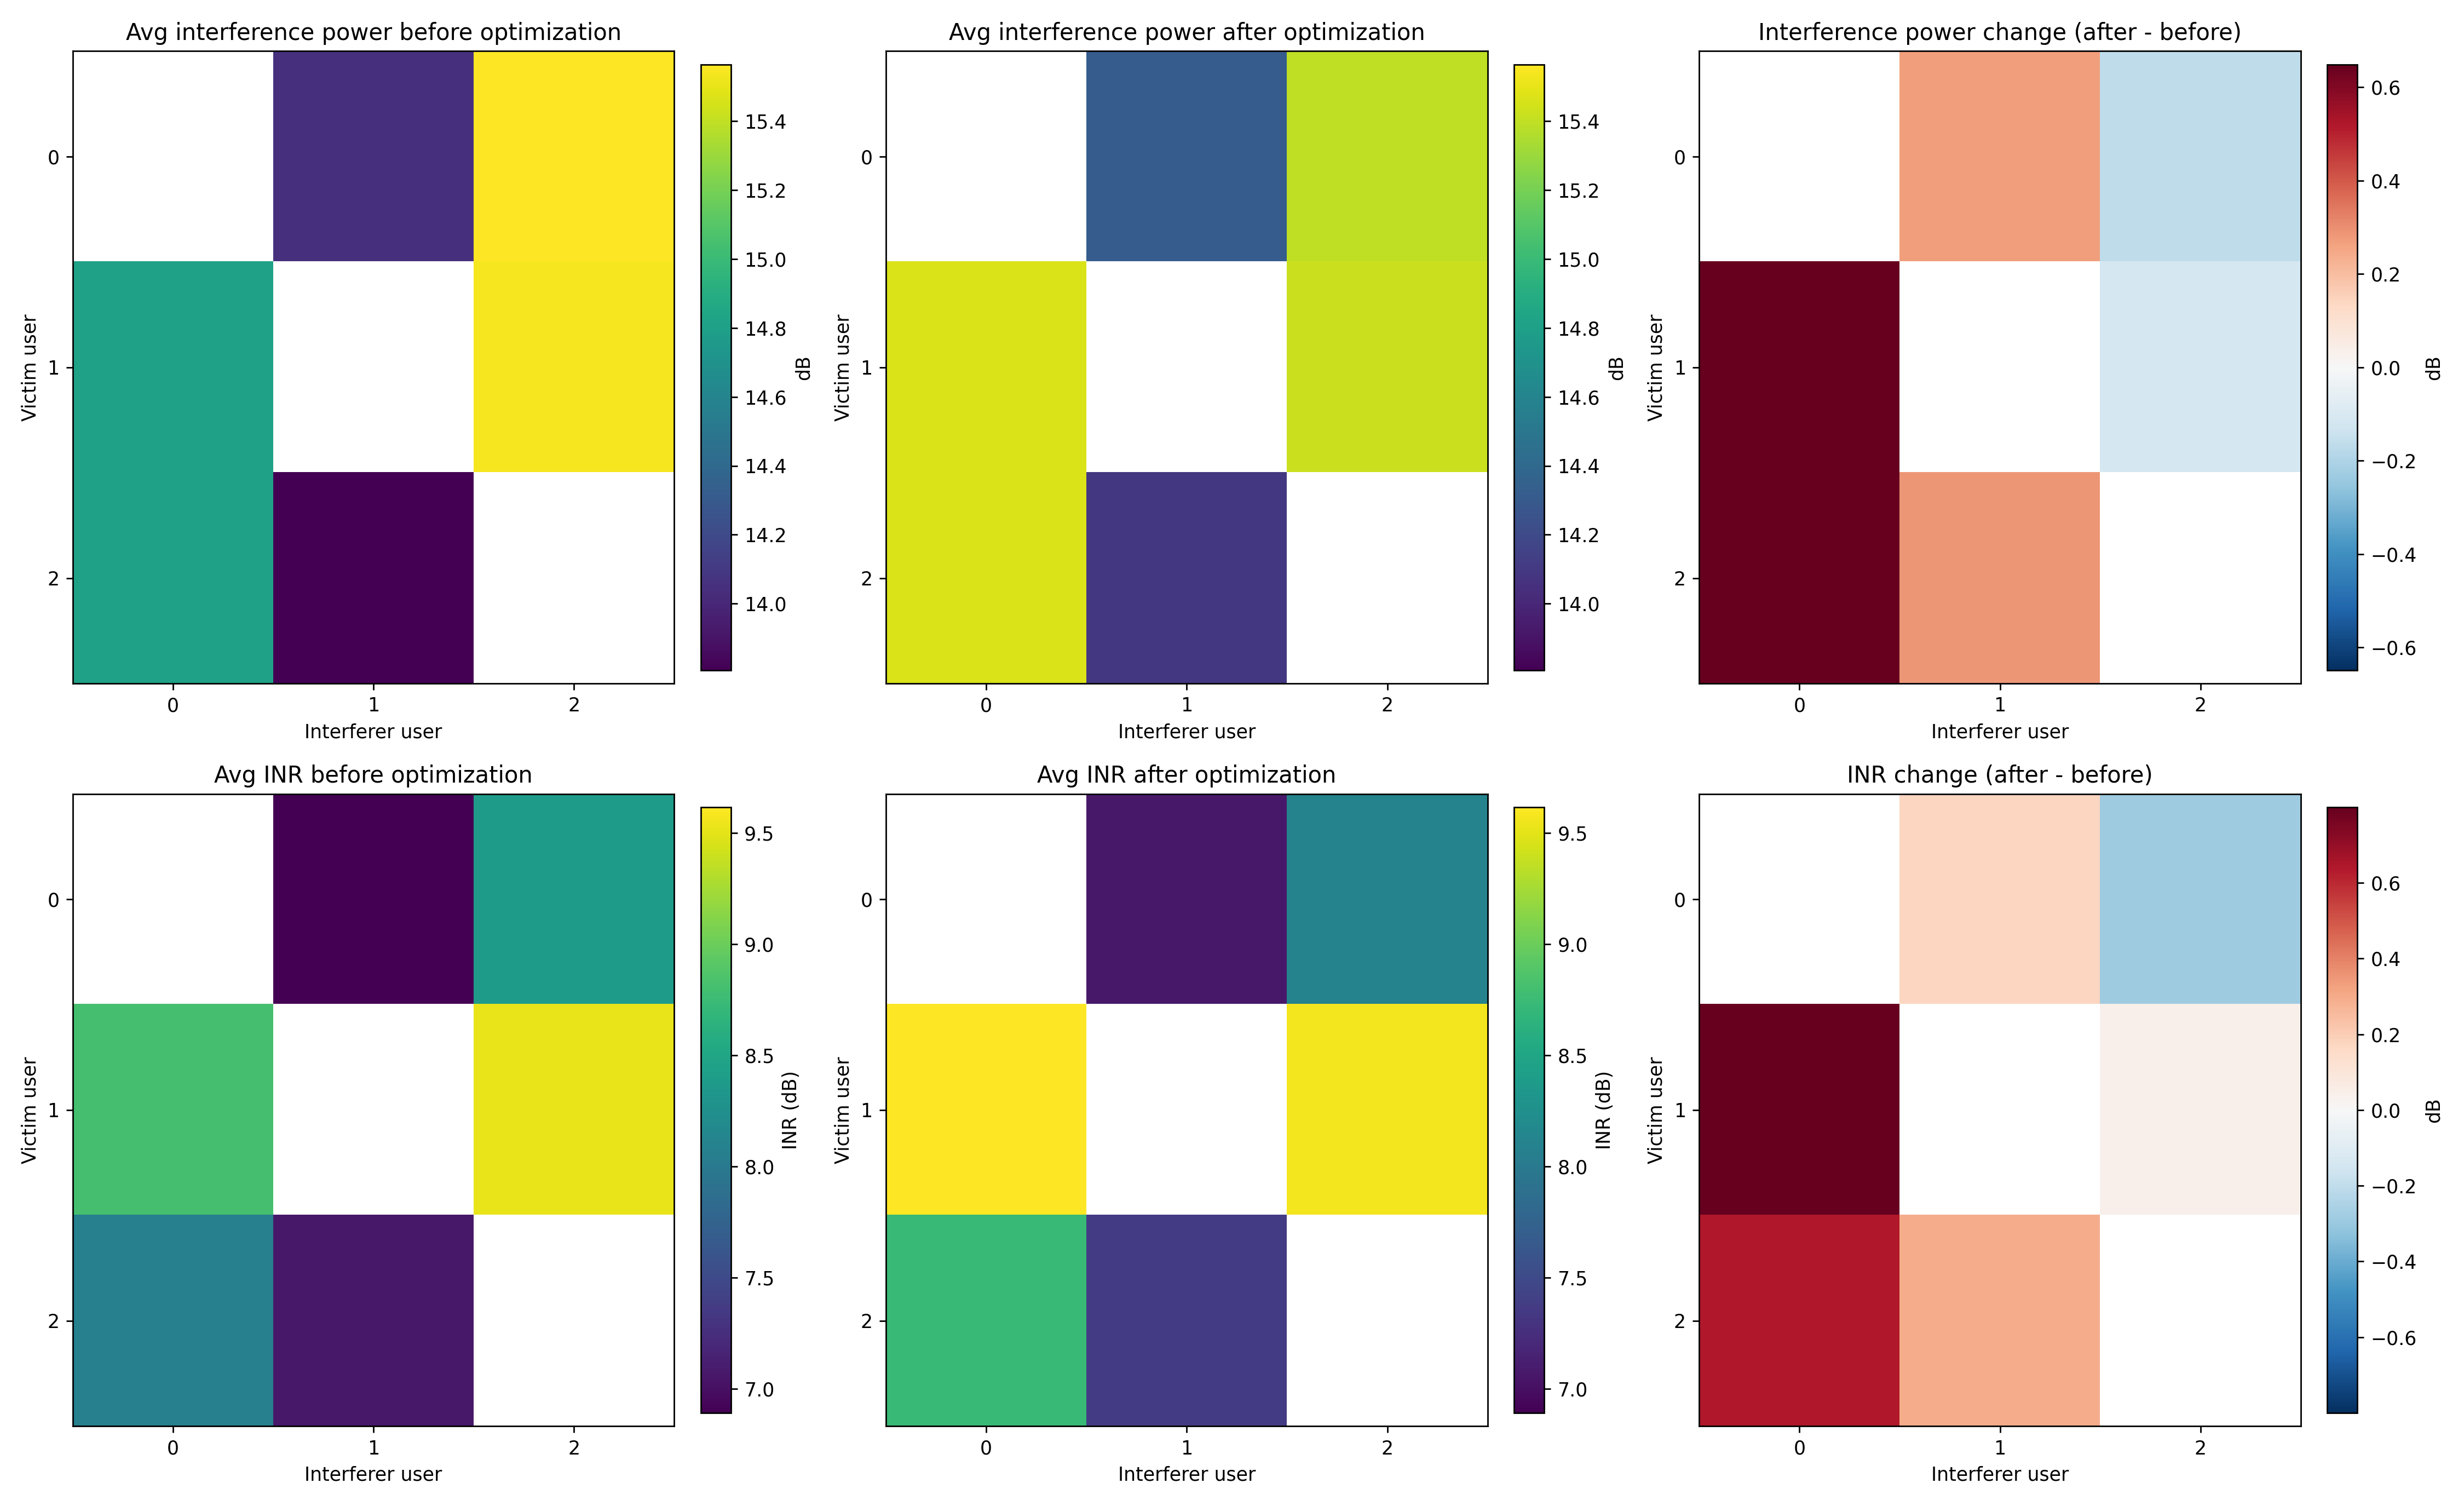
\includegraphics[width=\textwidth]{ul_payload_training_testing__interference_before_after_heatmaps.png}
    \caption{Training + Testing Method}
\end{subfigure}
\caption{Uplink payload-completion before/after heatmap comparison.}
\end{figure}

\section{Downlink Payload Completion}

The downlink payload-completion interference results are more structural. The
benchmark clears users from the active set more decisively, and that shows up
in both the \(-300\) dB inactive segments and the shorter schedule tail.

\begin{table}[H]
\centering
\small
\caption{Downlink payload-completion per-user served-block SINR summary}
\renewcommand{\arraystretch}{1.15}
\begin{tabularx}{\textwidth}{>{\centering\arraybackslash}p{0.10\textwidth} >{\centering\arraybackslash}p{0.18\textwidth} >{\centering\arraybackslash}p{0.18\textwidth} X}
\toprule
User & Training Only init/final & Training + Testing init/final & Reading \\
\midrule
0 & \(-3.003/18.920\) dB & \(-3.003/14.017\) dB & Benchmark is much stronger after skipped-block concentration. \\
1 & \(-2.774/10.052\) dB & \(-2.774/13.141\) dB & Training + Testing is stronger on this easier user. \\
2 & \(-2.764/12.894\) dB & \(-2.764/11.416\) dB & Benchmark is stronger and finishes earlier. \\
\bottomrule
\end{tabularx}
\end{table}

\begin{figure}[H]
\centering
\begin{subfigure}[t]{0.48\textwidth}
    \centering
    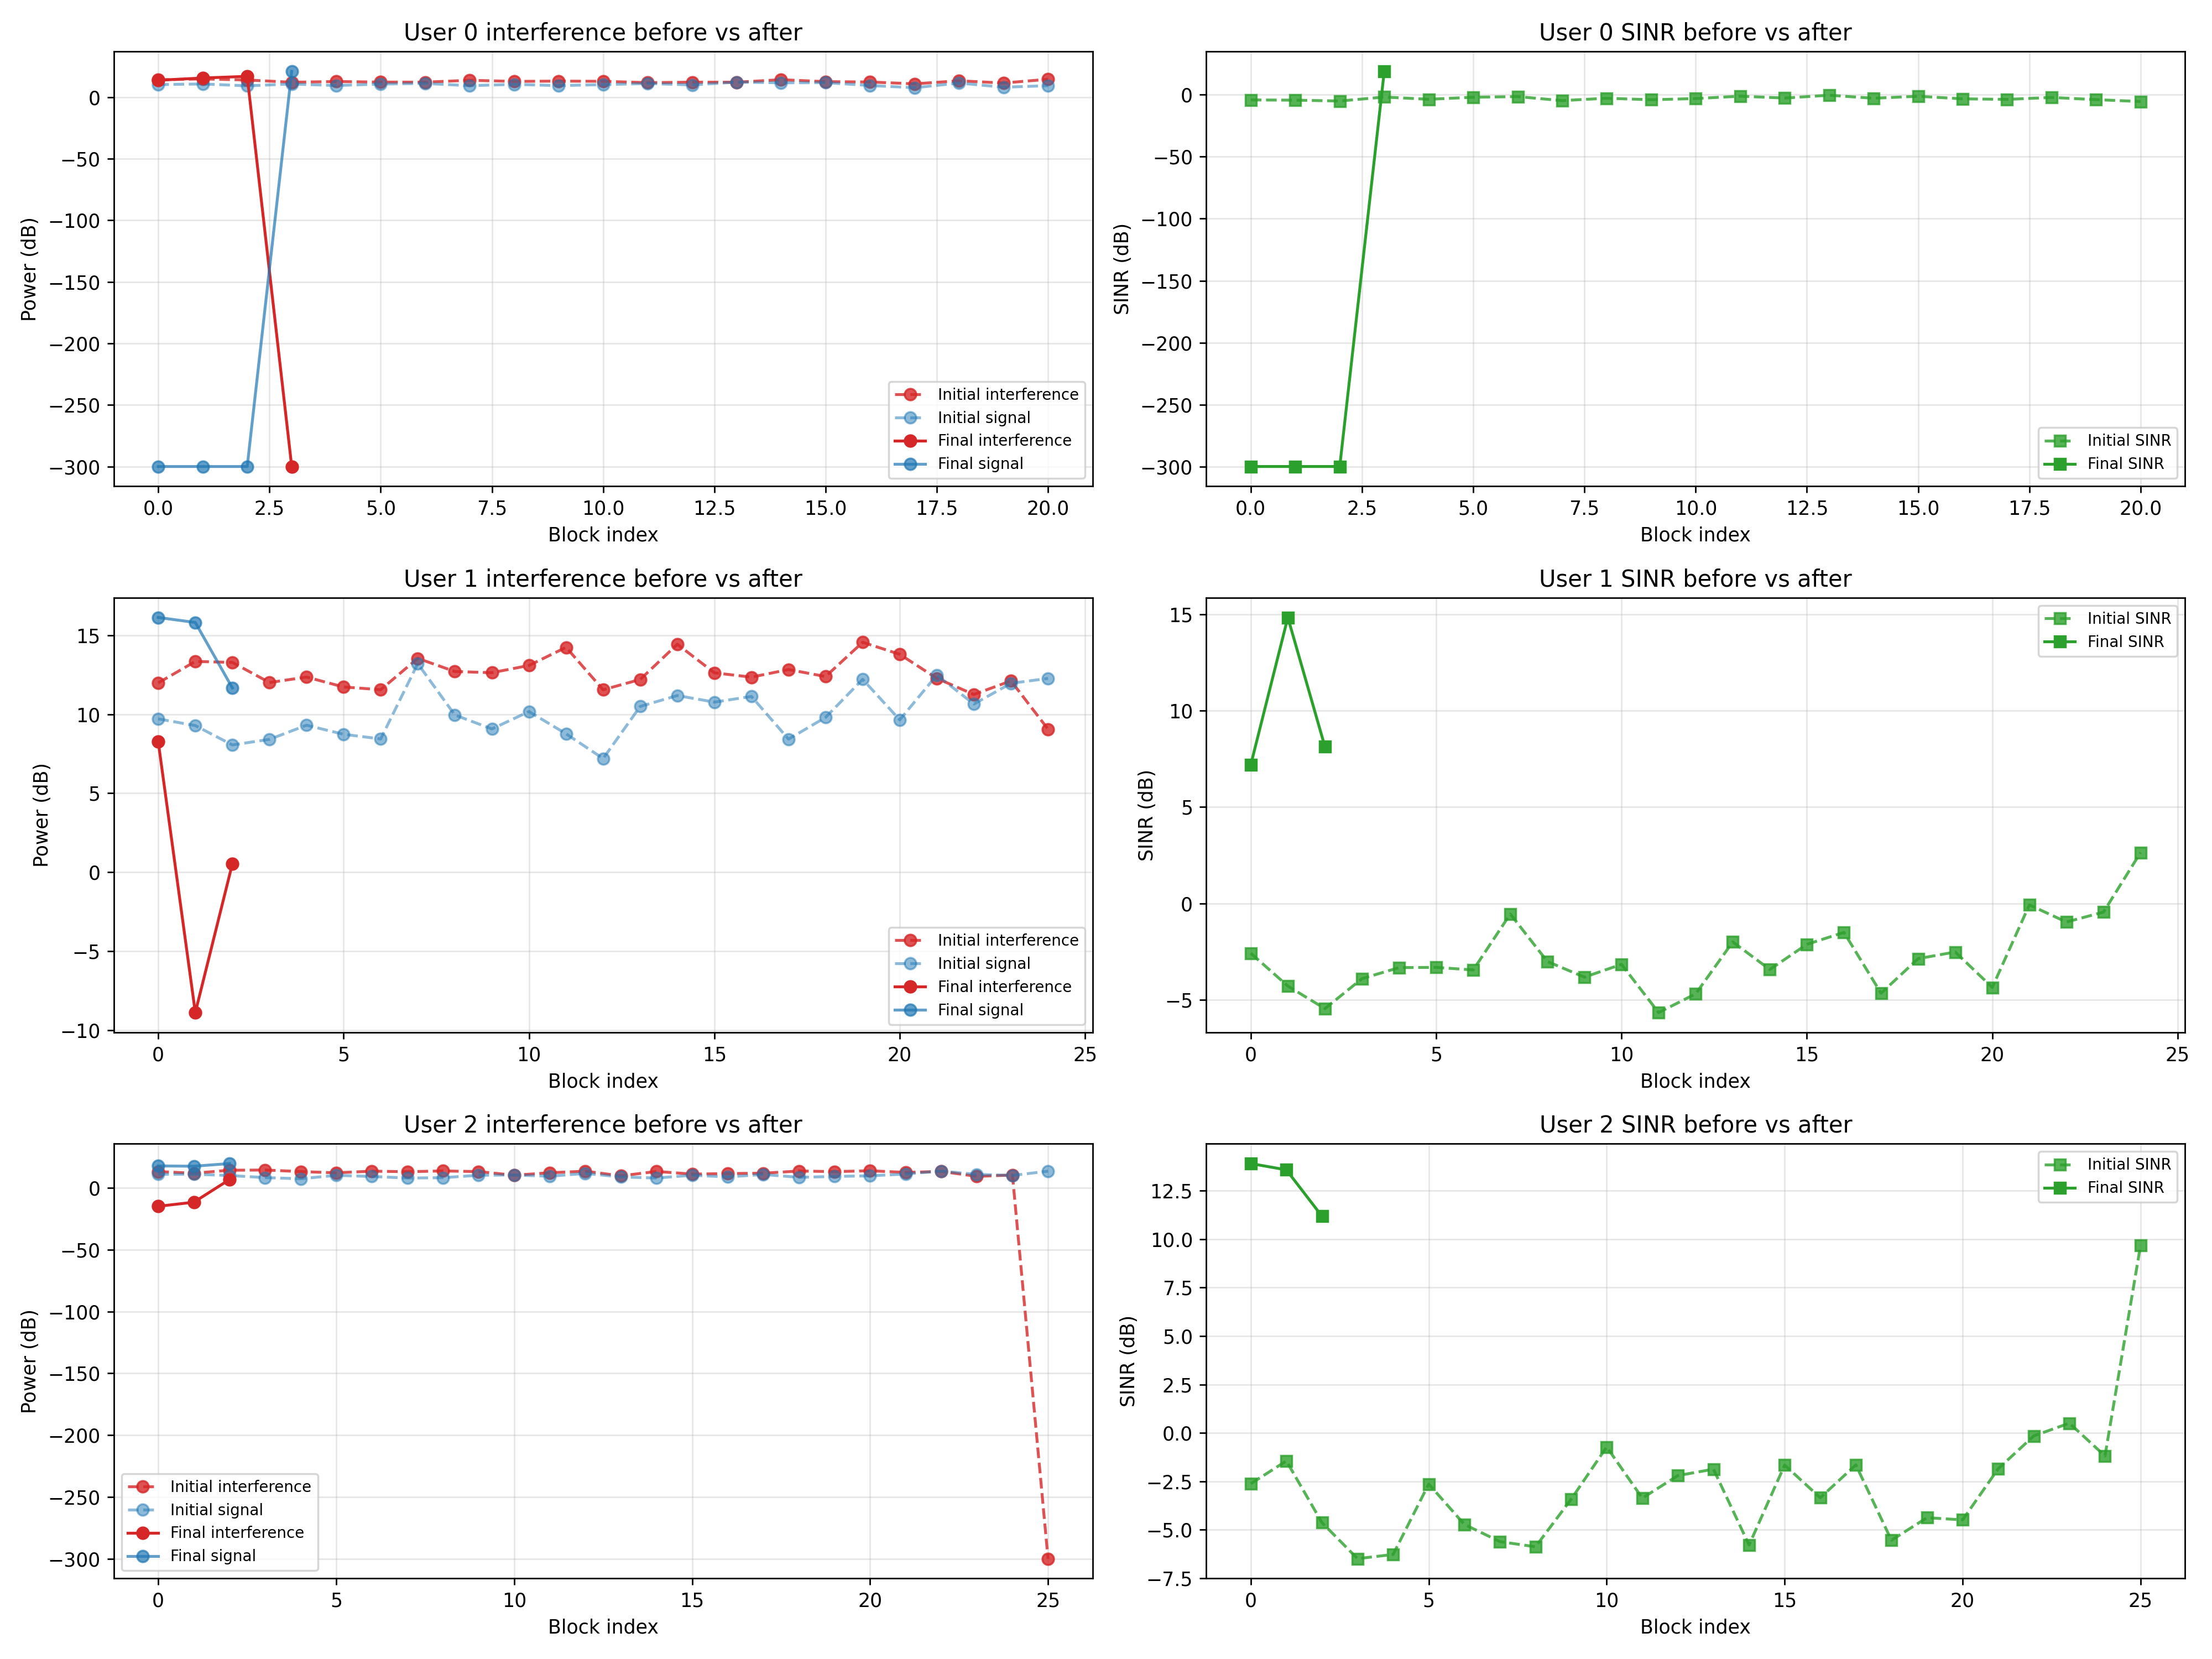
\includegraphics[width=\textwidth]{dl_payload_training_only__per_user_interference_before_after.png}
    \caption{Training Only Method}
\end{subfigure}
\hfill
\begin{subfigure}[t]{0.48\textwidth}
    \centering
    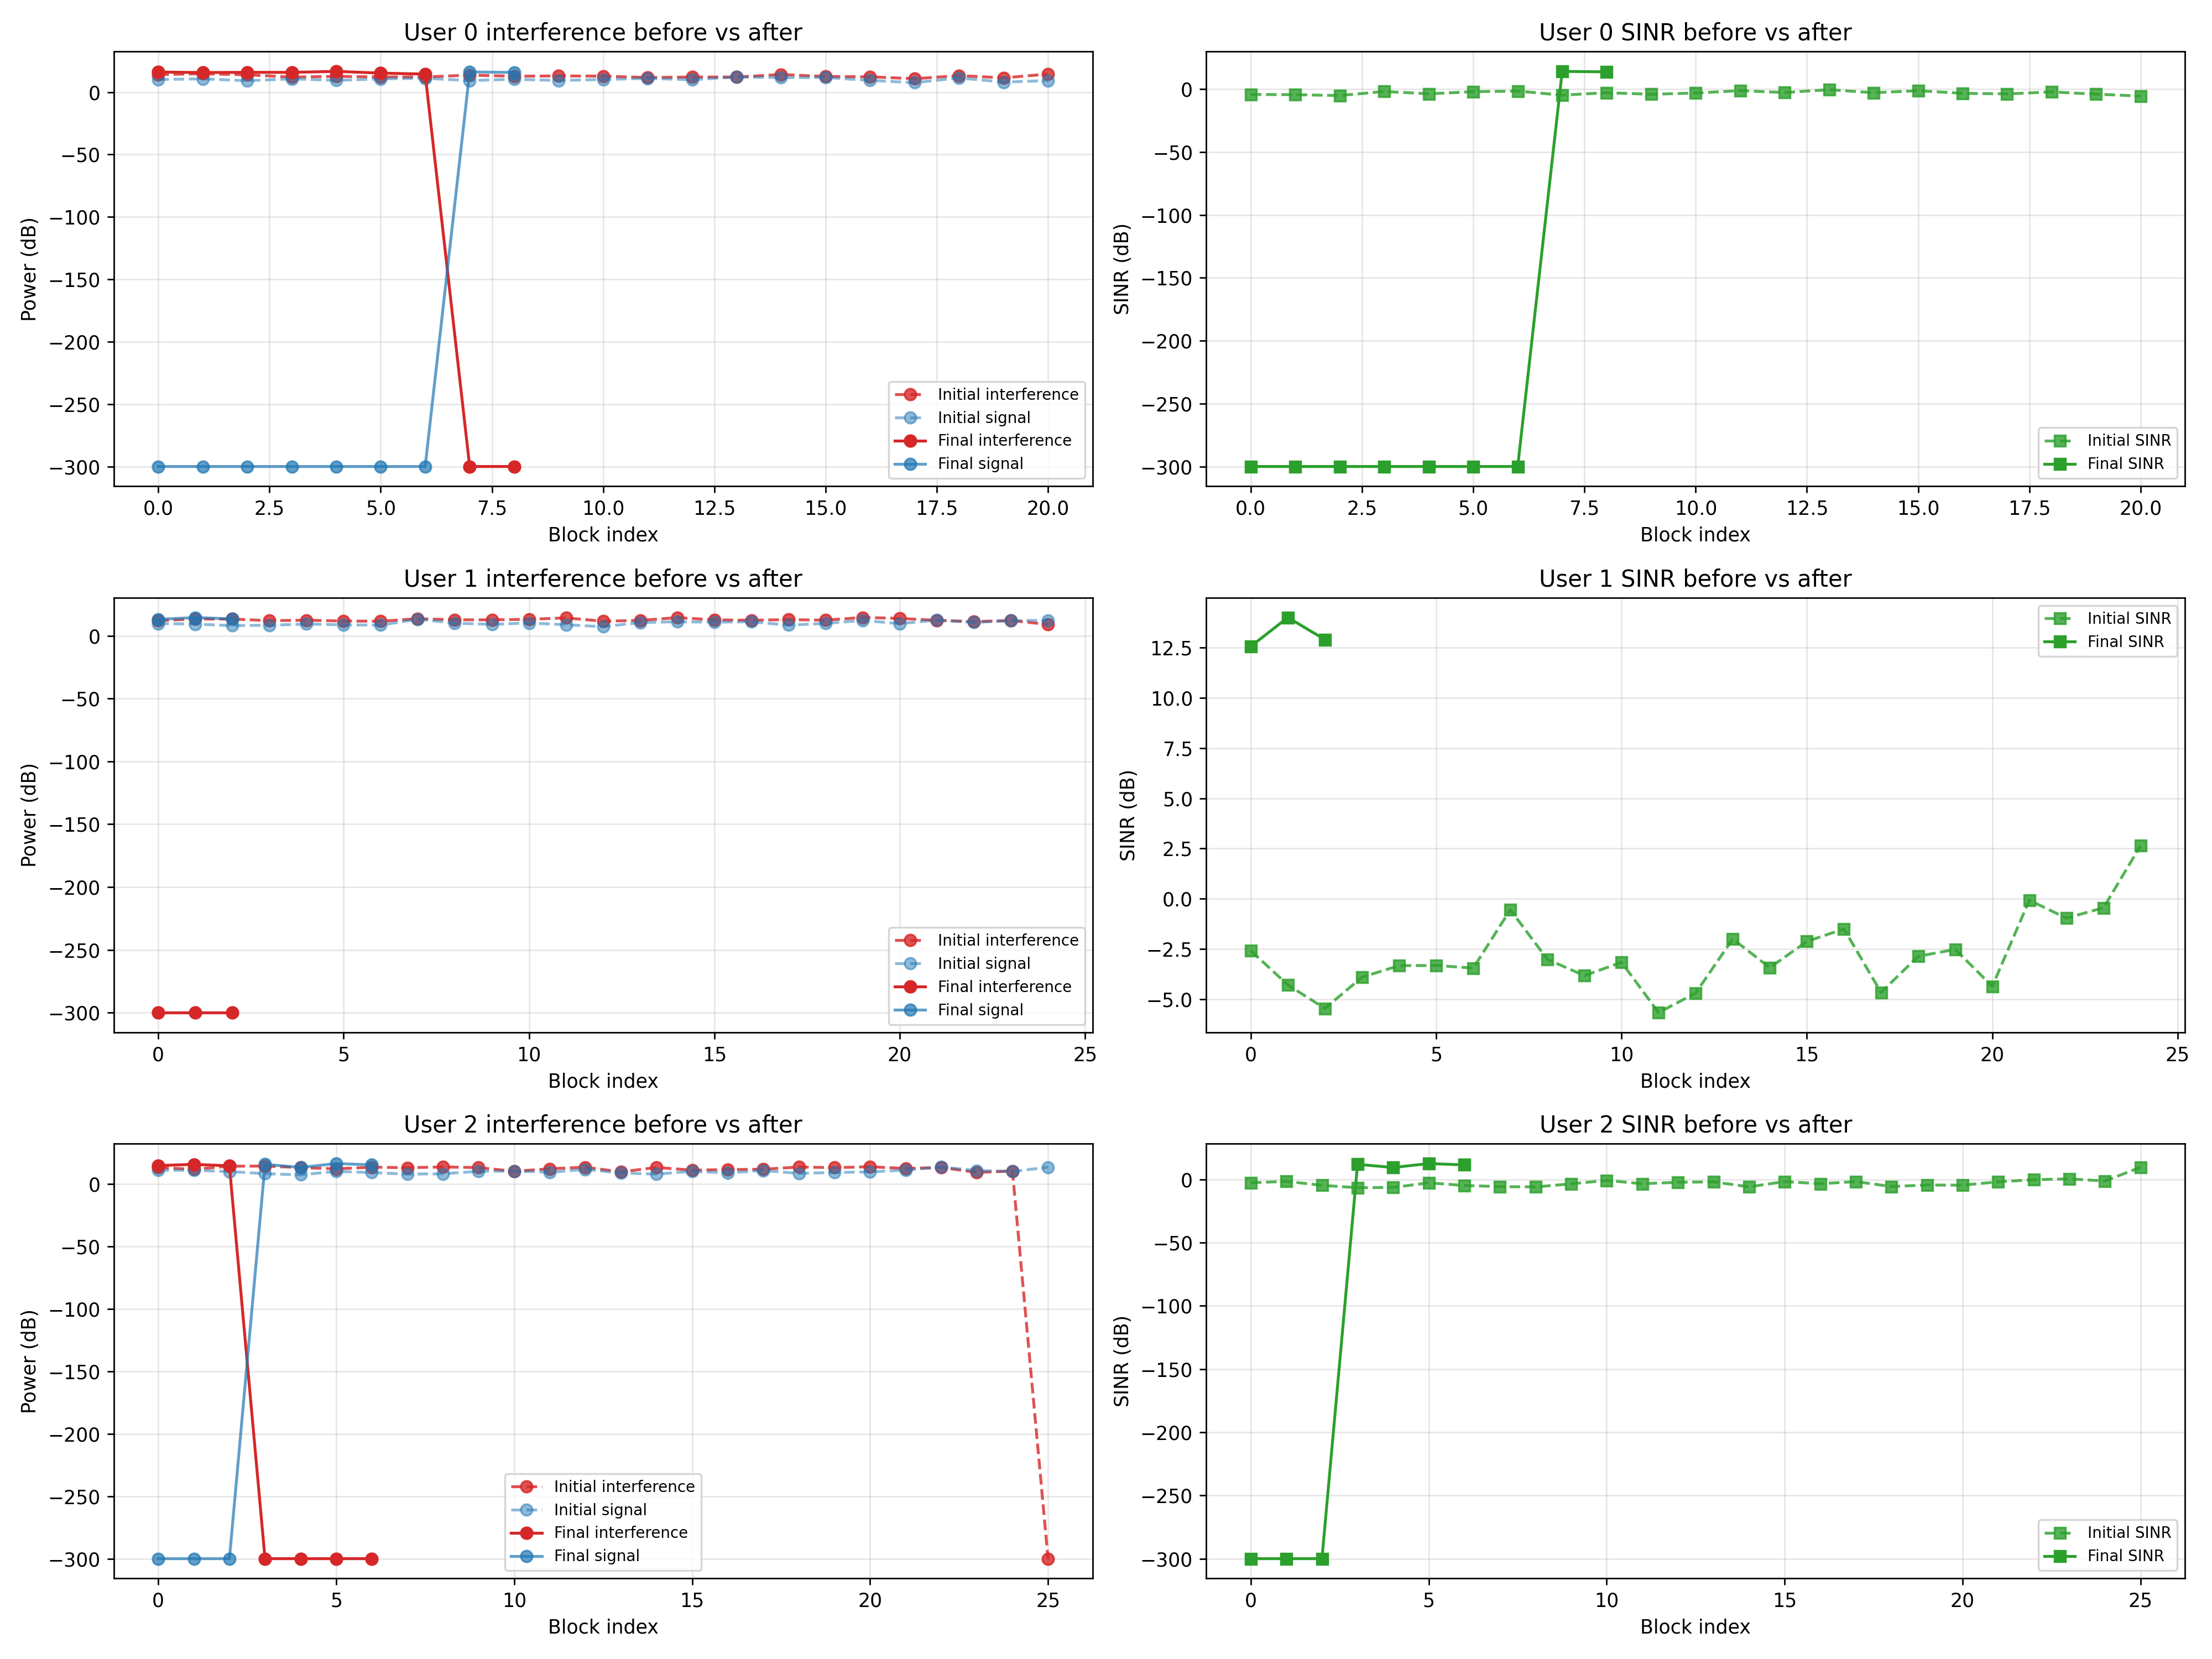
\includegraphics[width=\textwidth]{dl_payload_training_testing__per_user_interference_before_after.png}
    \caption{Training + Testing Method}
\end{subfigure}
\caption{Downlink payload-completion per-user interference before/after comparison.}
\end{figure}

\begin{figure}[H]
\centering
\begin{subfigure}[t]{0.48\textwidth}
    \centering
    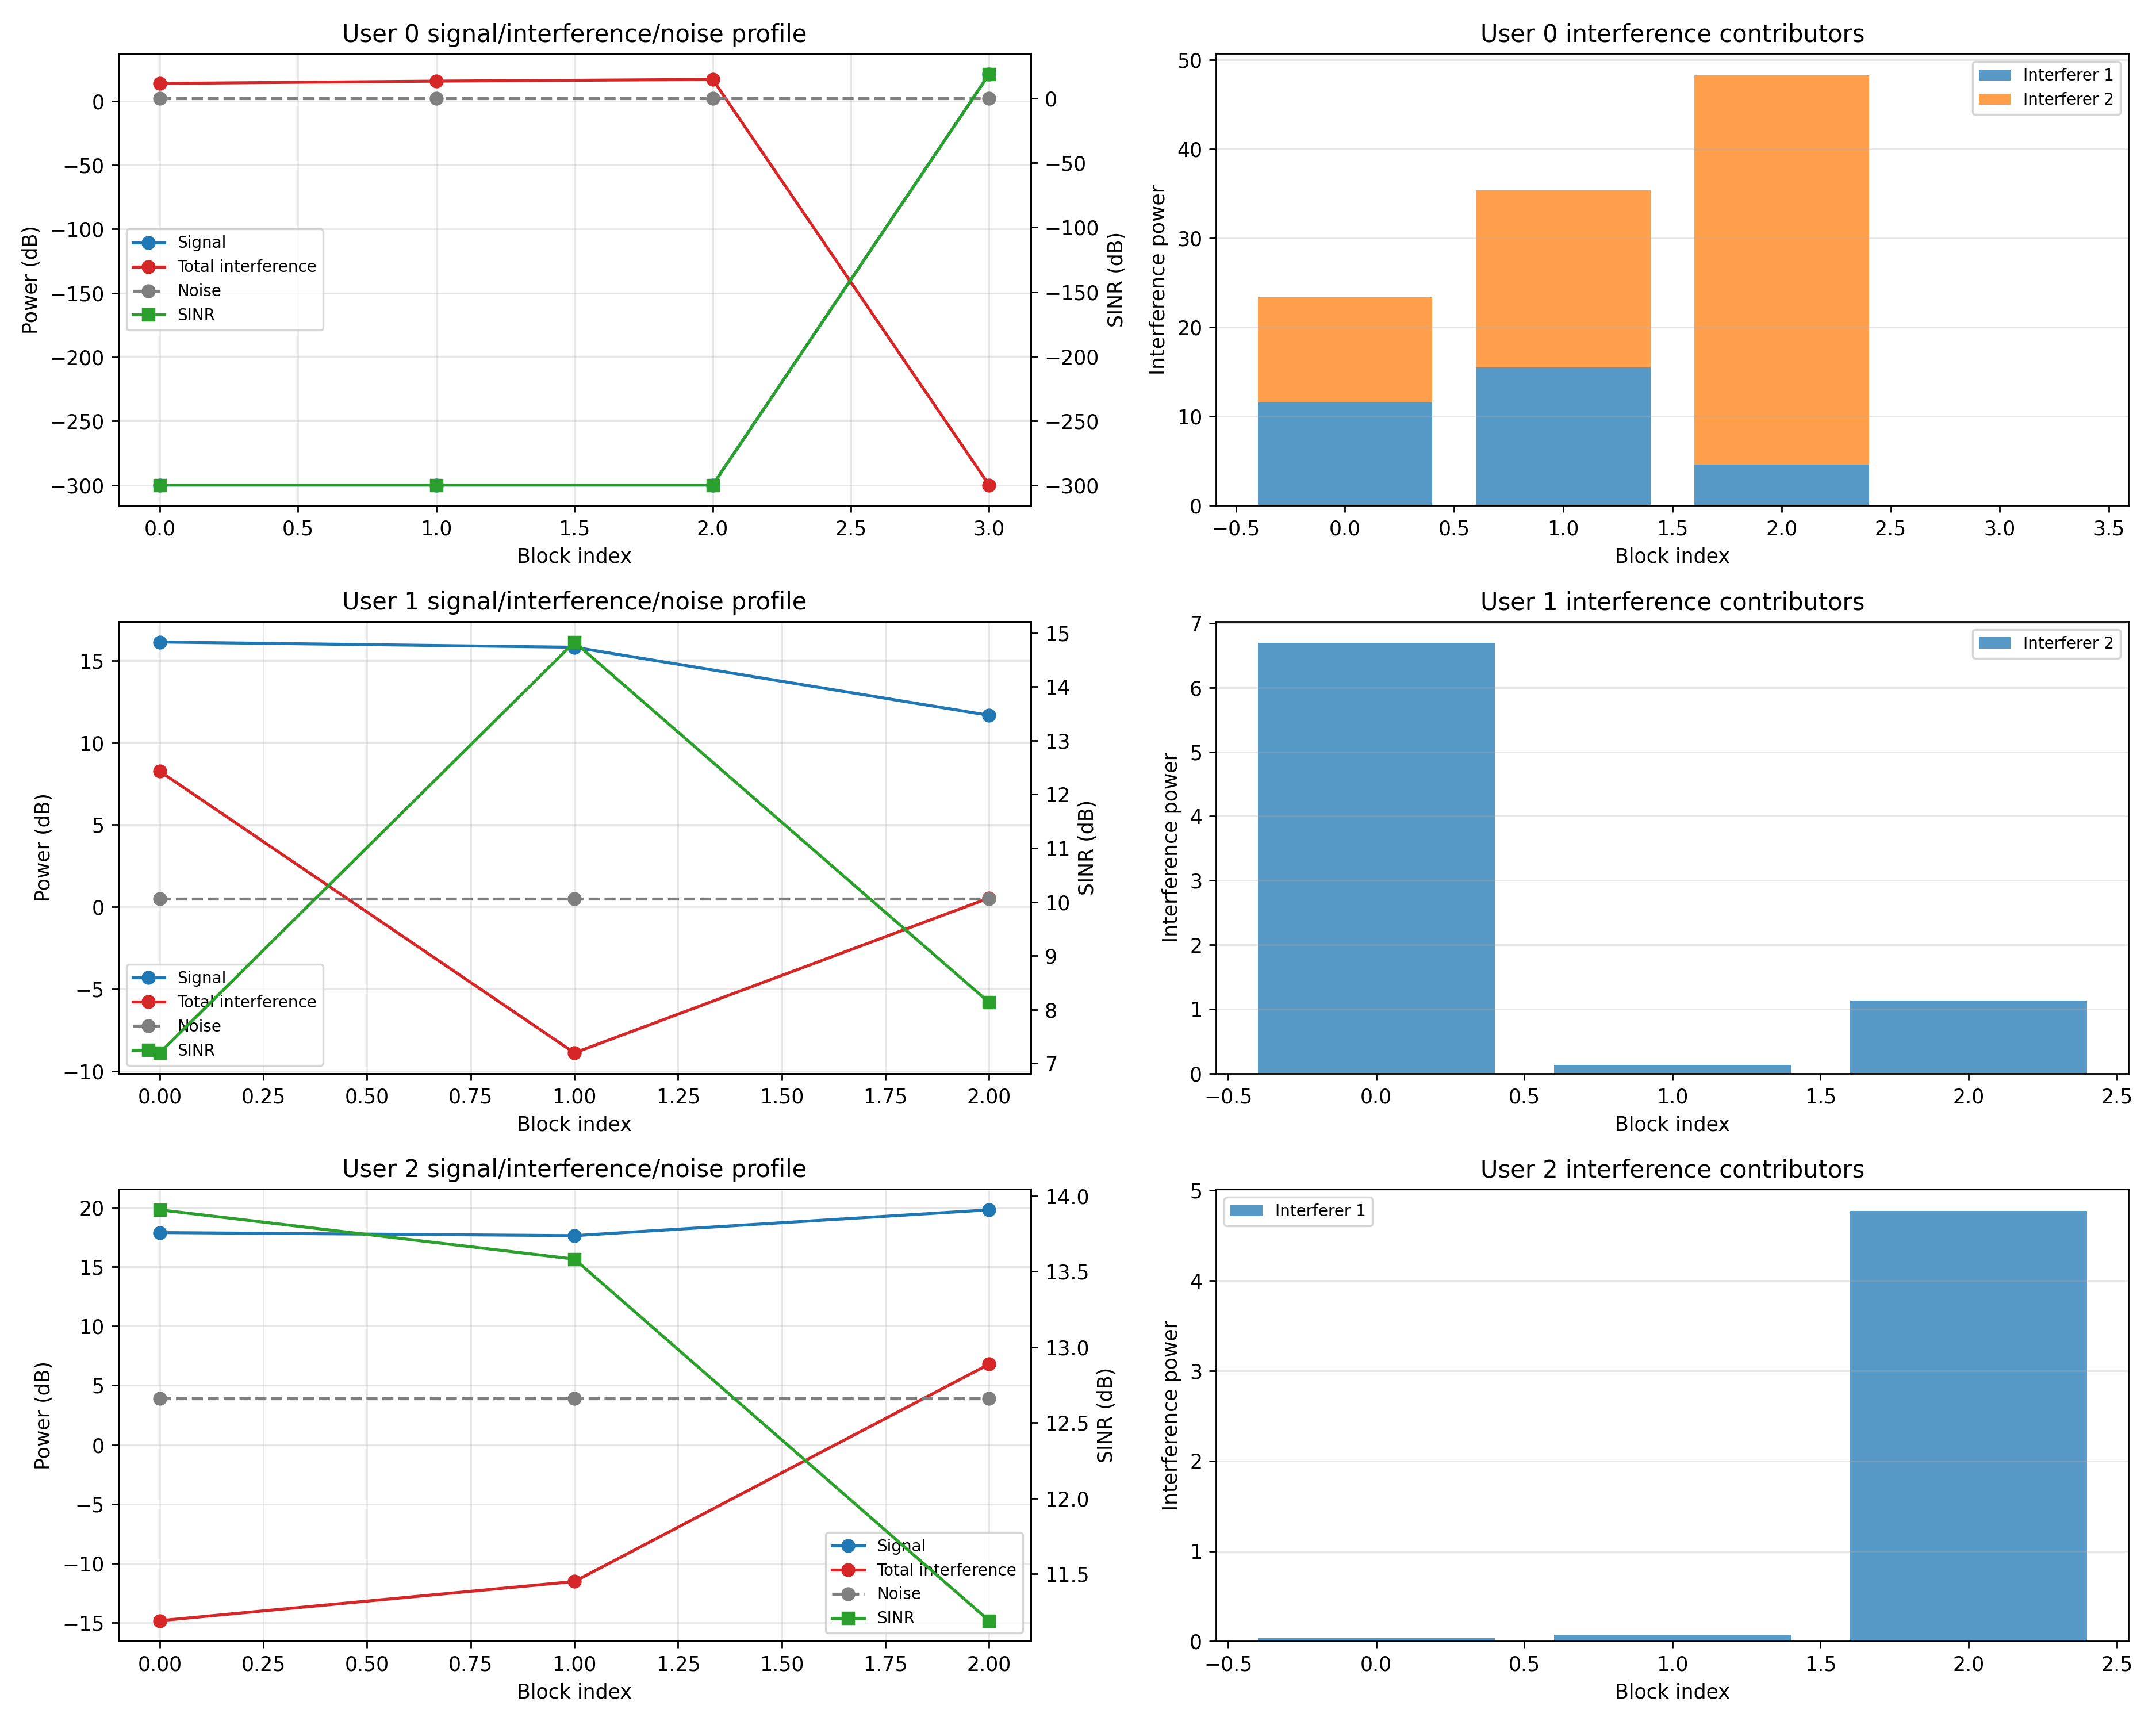
\includegraphics[width=\textwidth]{dl_payload_training_only__per_user_interference_profiles.png}
    \caption{Training Only Method}
\end{subfigure}
\hfill
\begin{subfigure}[t]{0.48\textwidth}
    \centering
    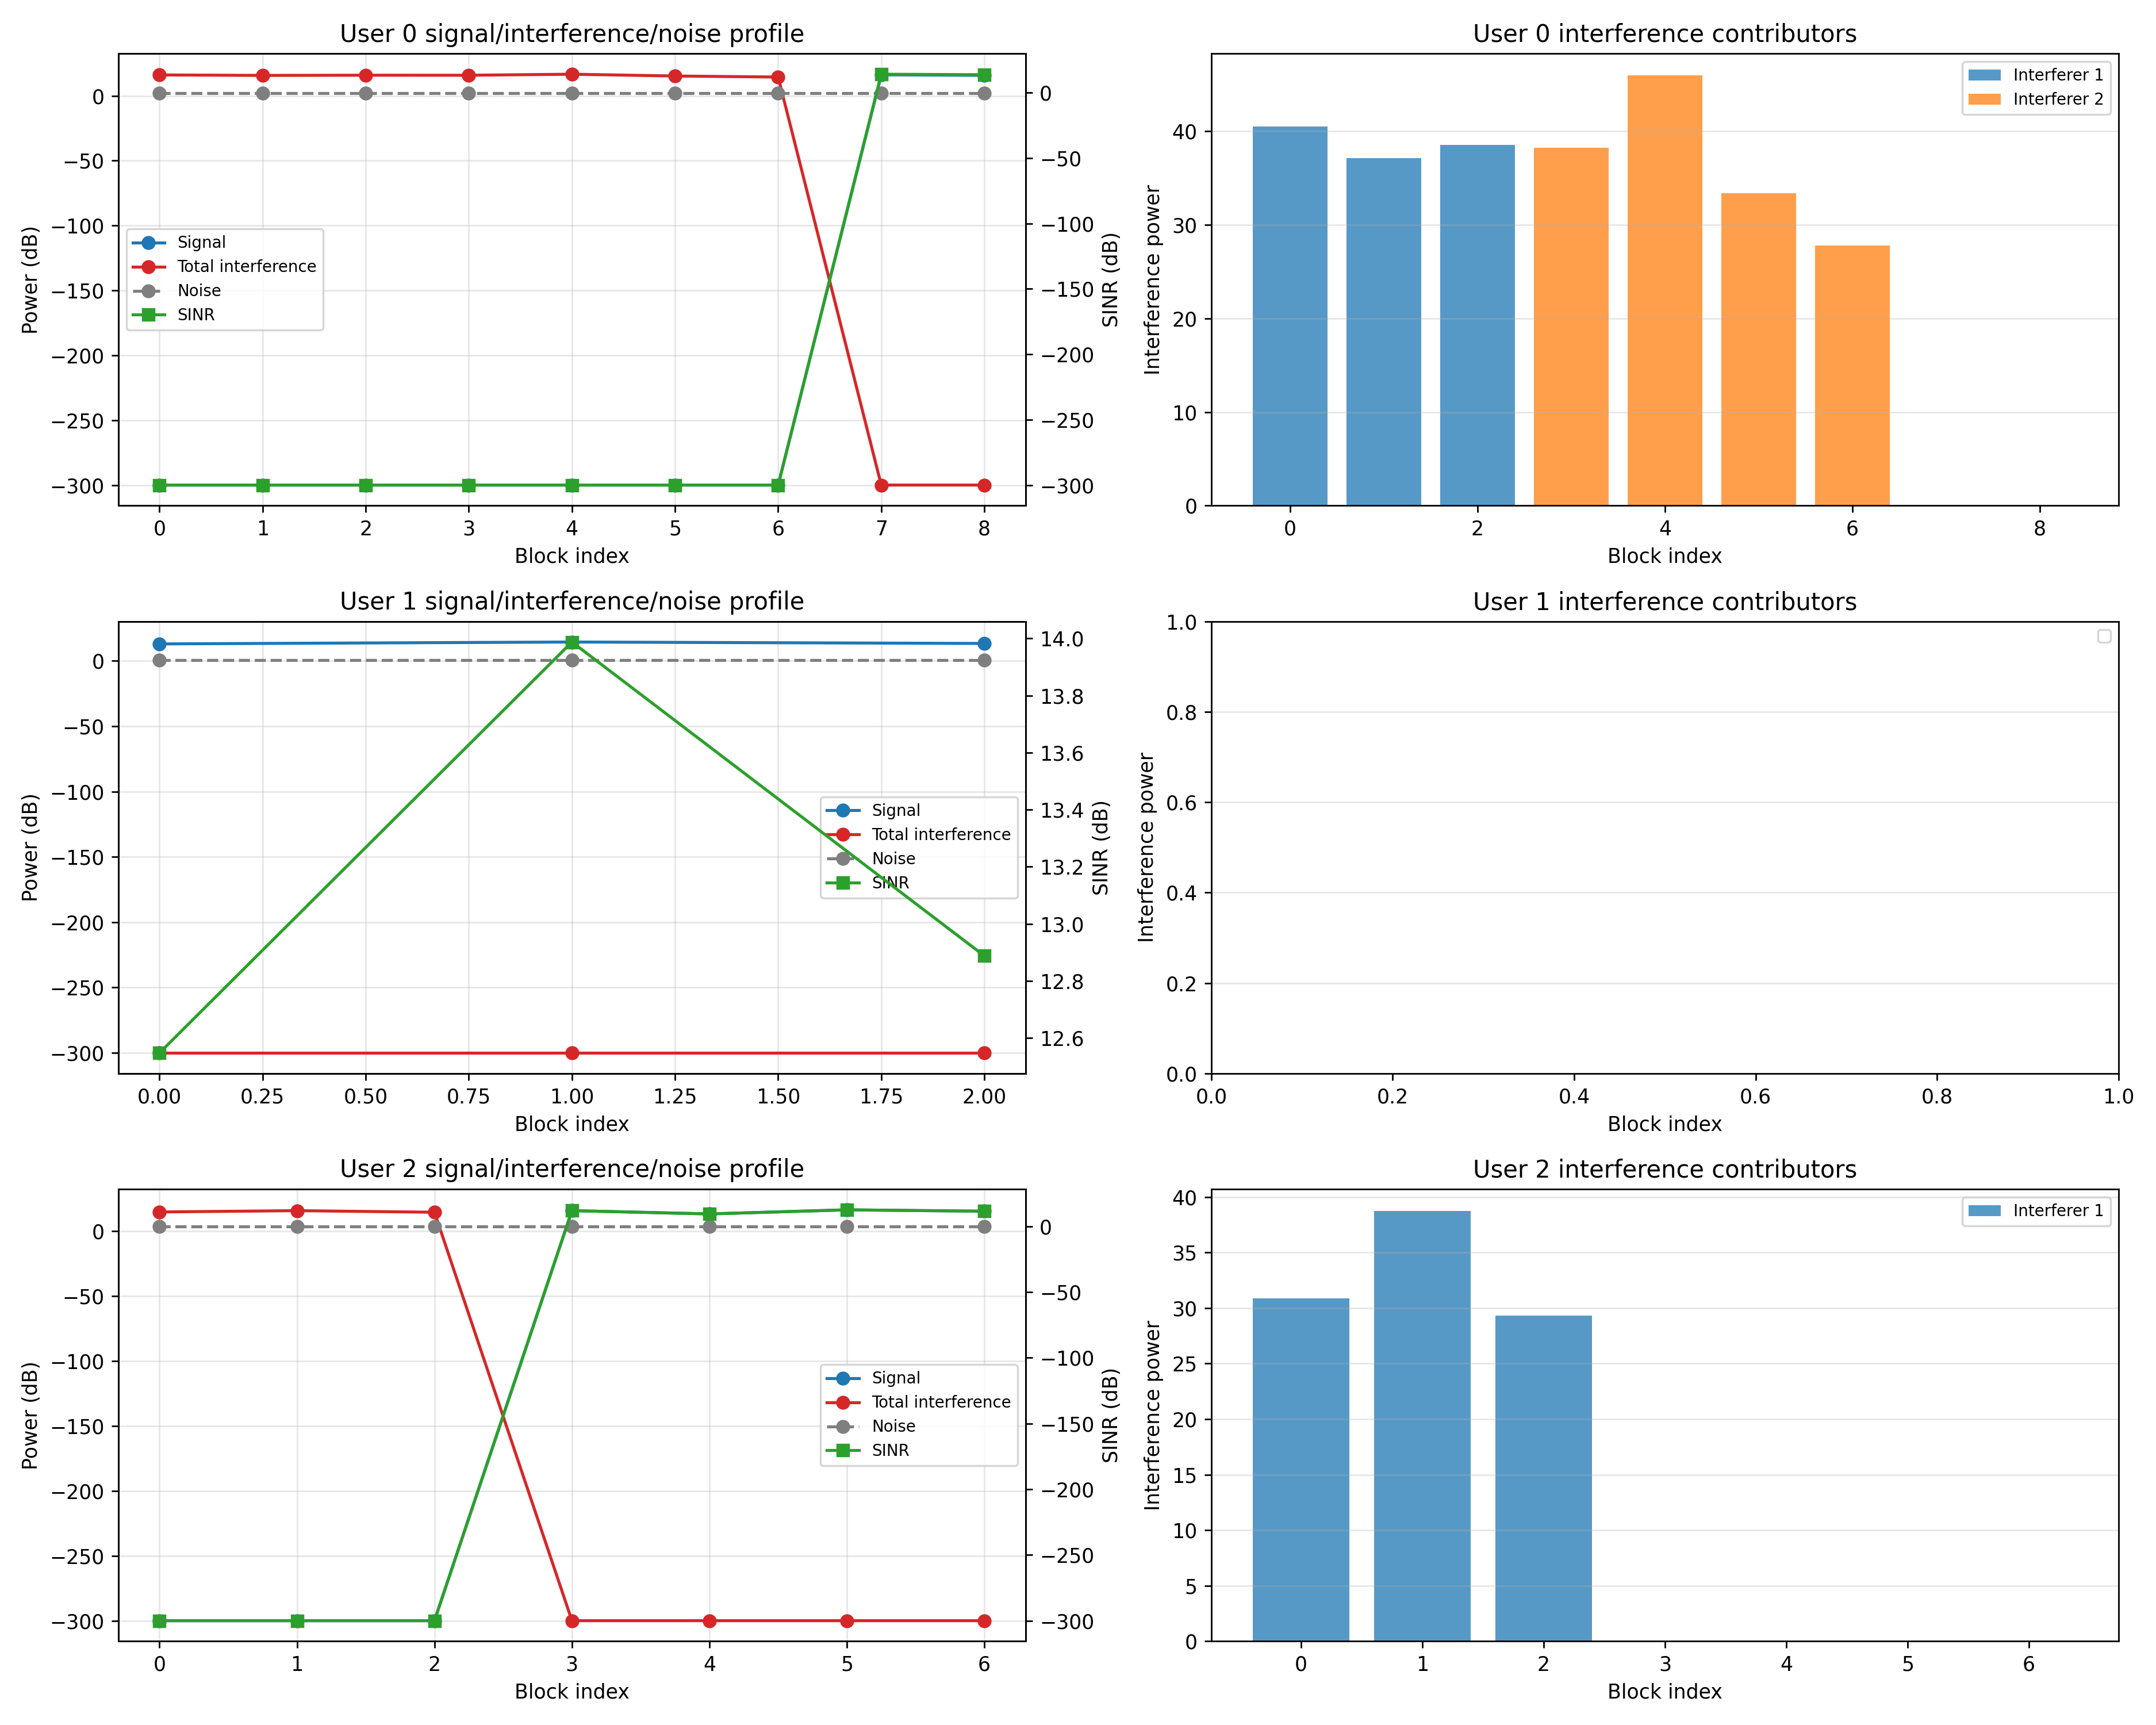
\includegraphics[width=\textwidth]{dl_payload_training_testing__per_user_interference_profiles.png}
    \caption{Training + Testing Method}
\end{subfigure}
\caption{Downlink payload-completion per-user interference profiles.}
\end{figure}

\begin{figure}[H]
\centering
\begin{subfigure}[t]{0.48\textwidth}
    \centering
    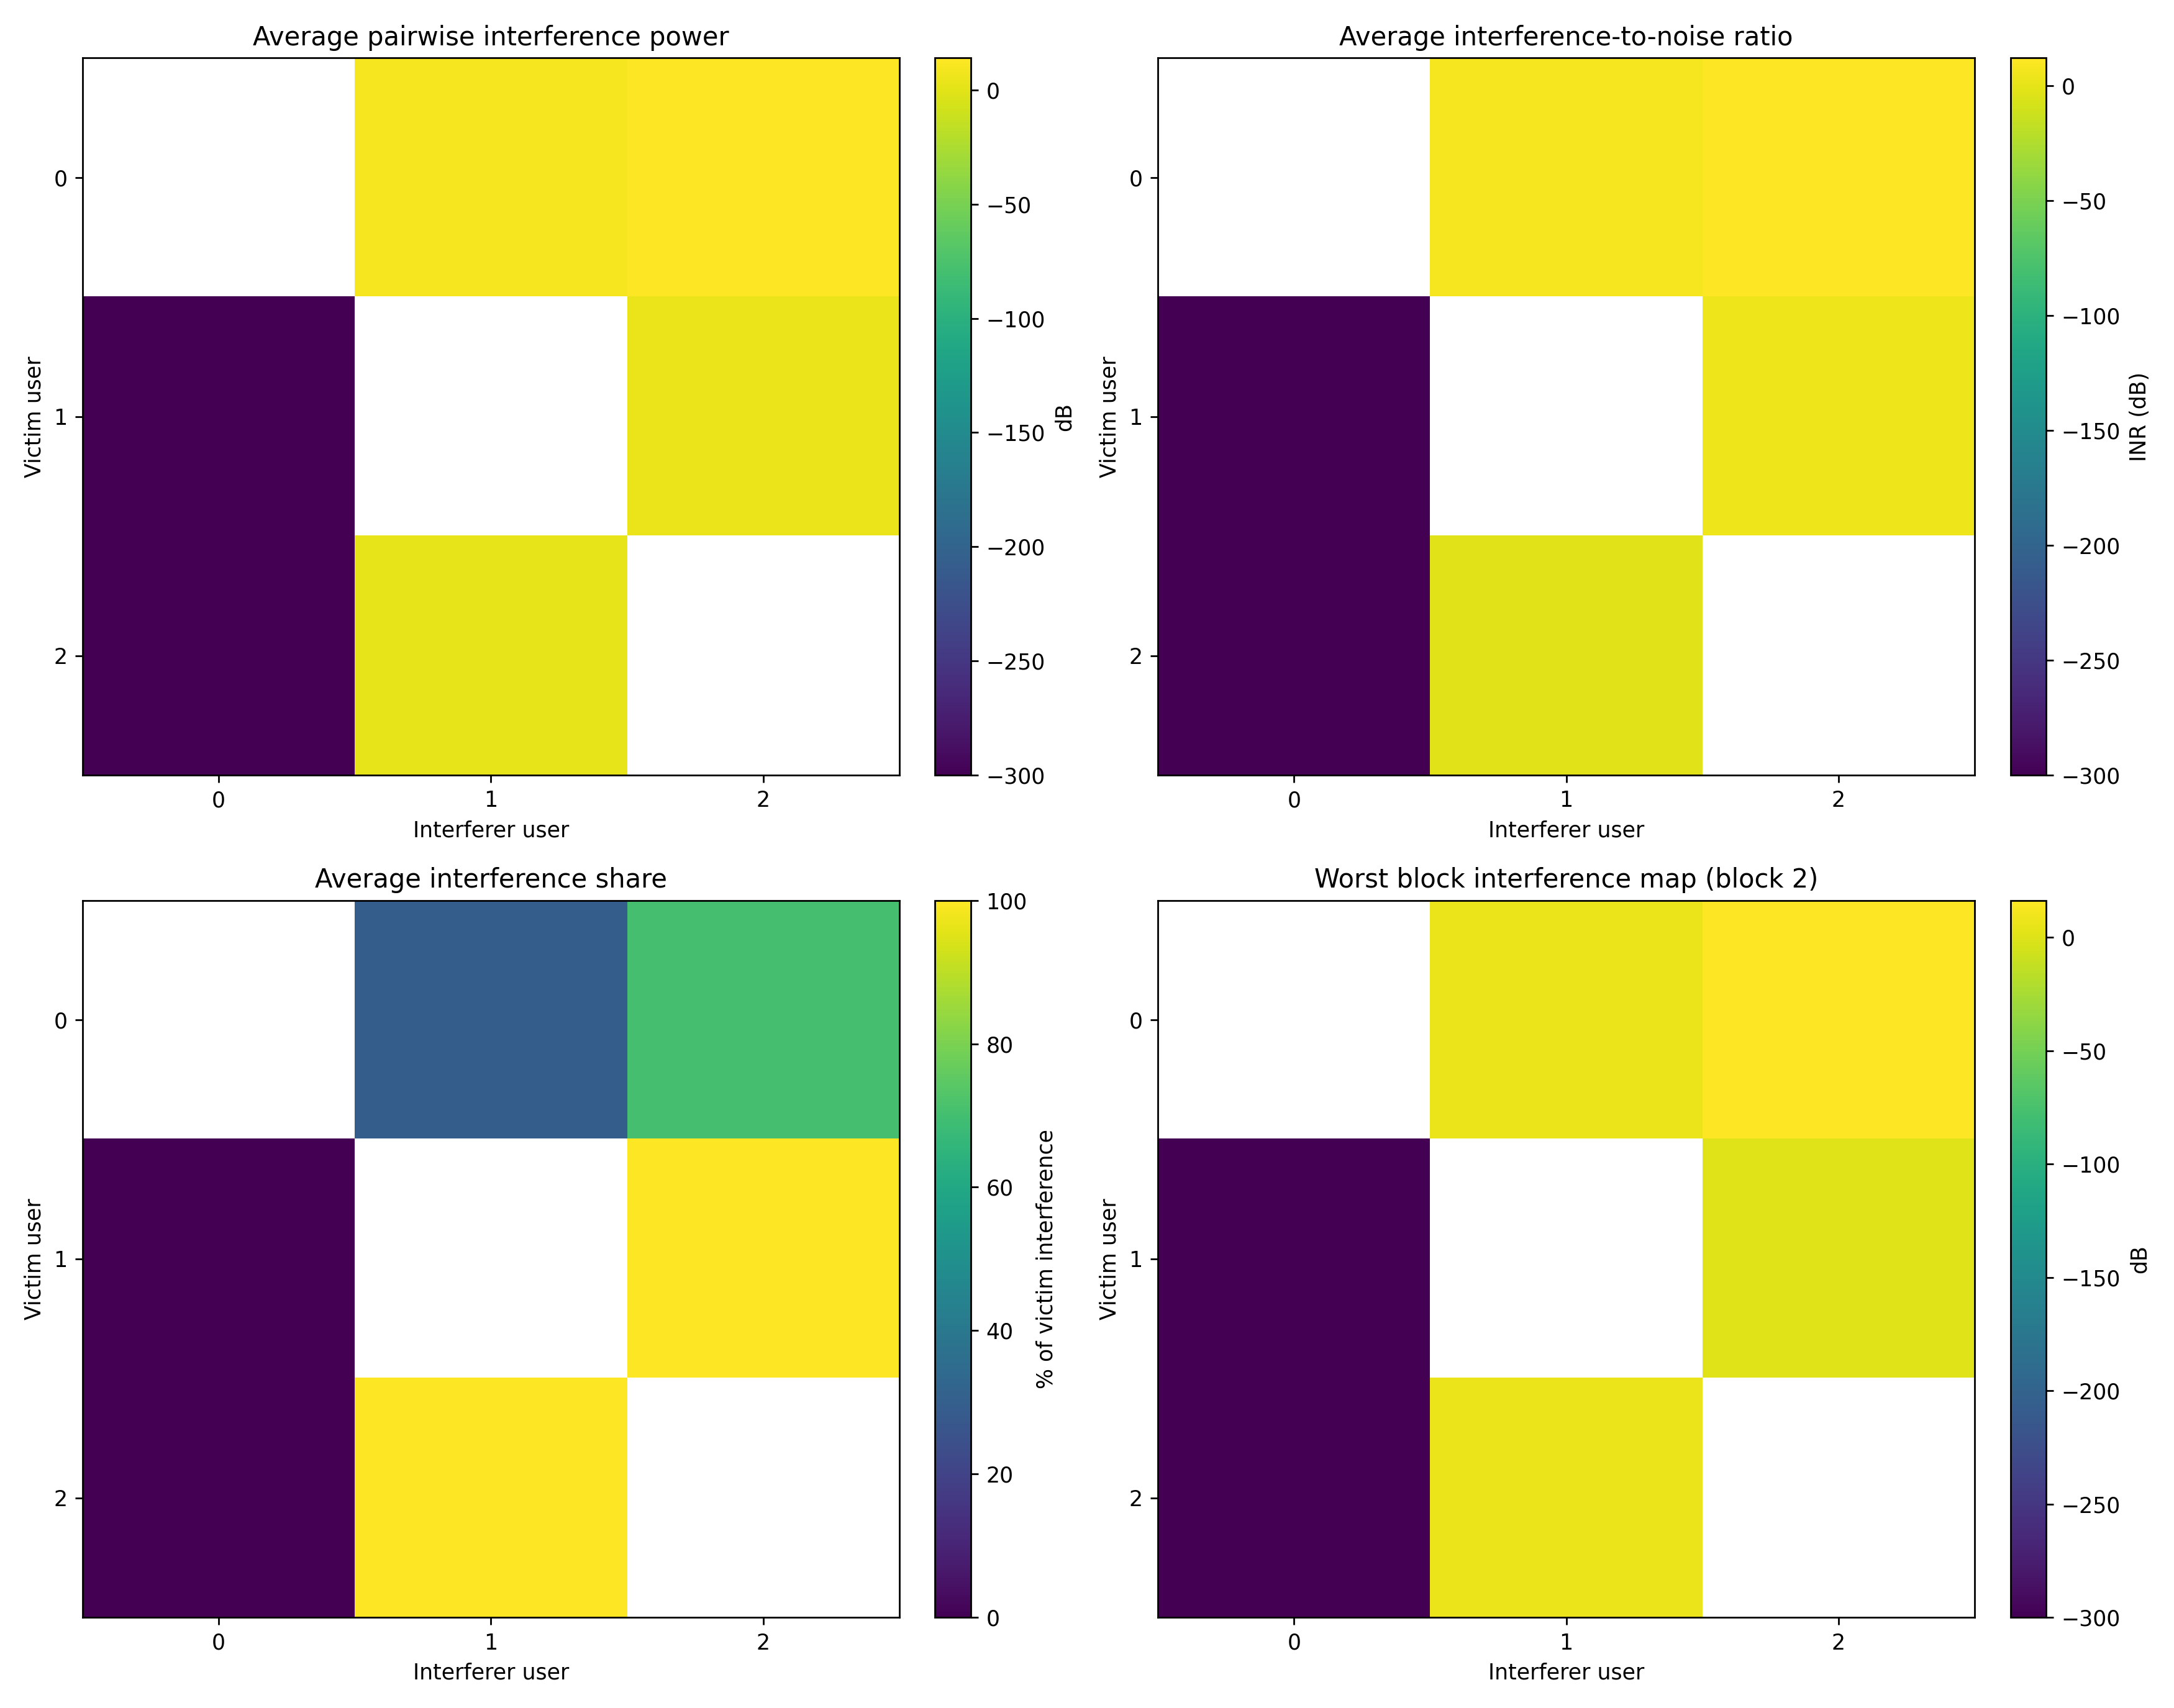
\includegraphics[width=\textwidth]{dl_payload_training_only__interference_heatmaps.png}
    \caption{Training Only Method}
\end{subfigure}
\hfill
\begin{subfigure}[t]{0.48\textwidth}
    \centering
    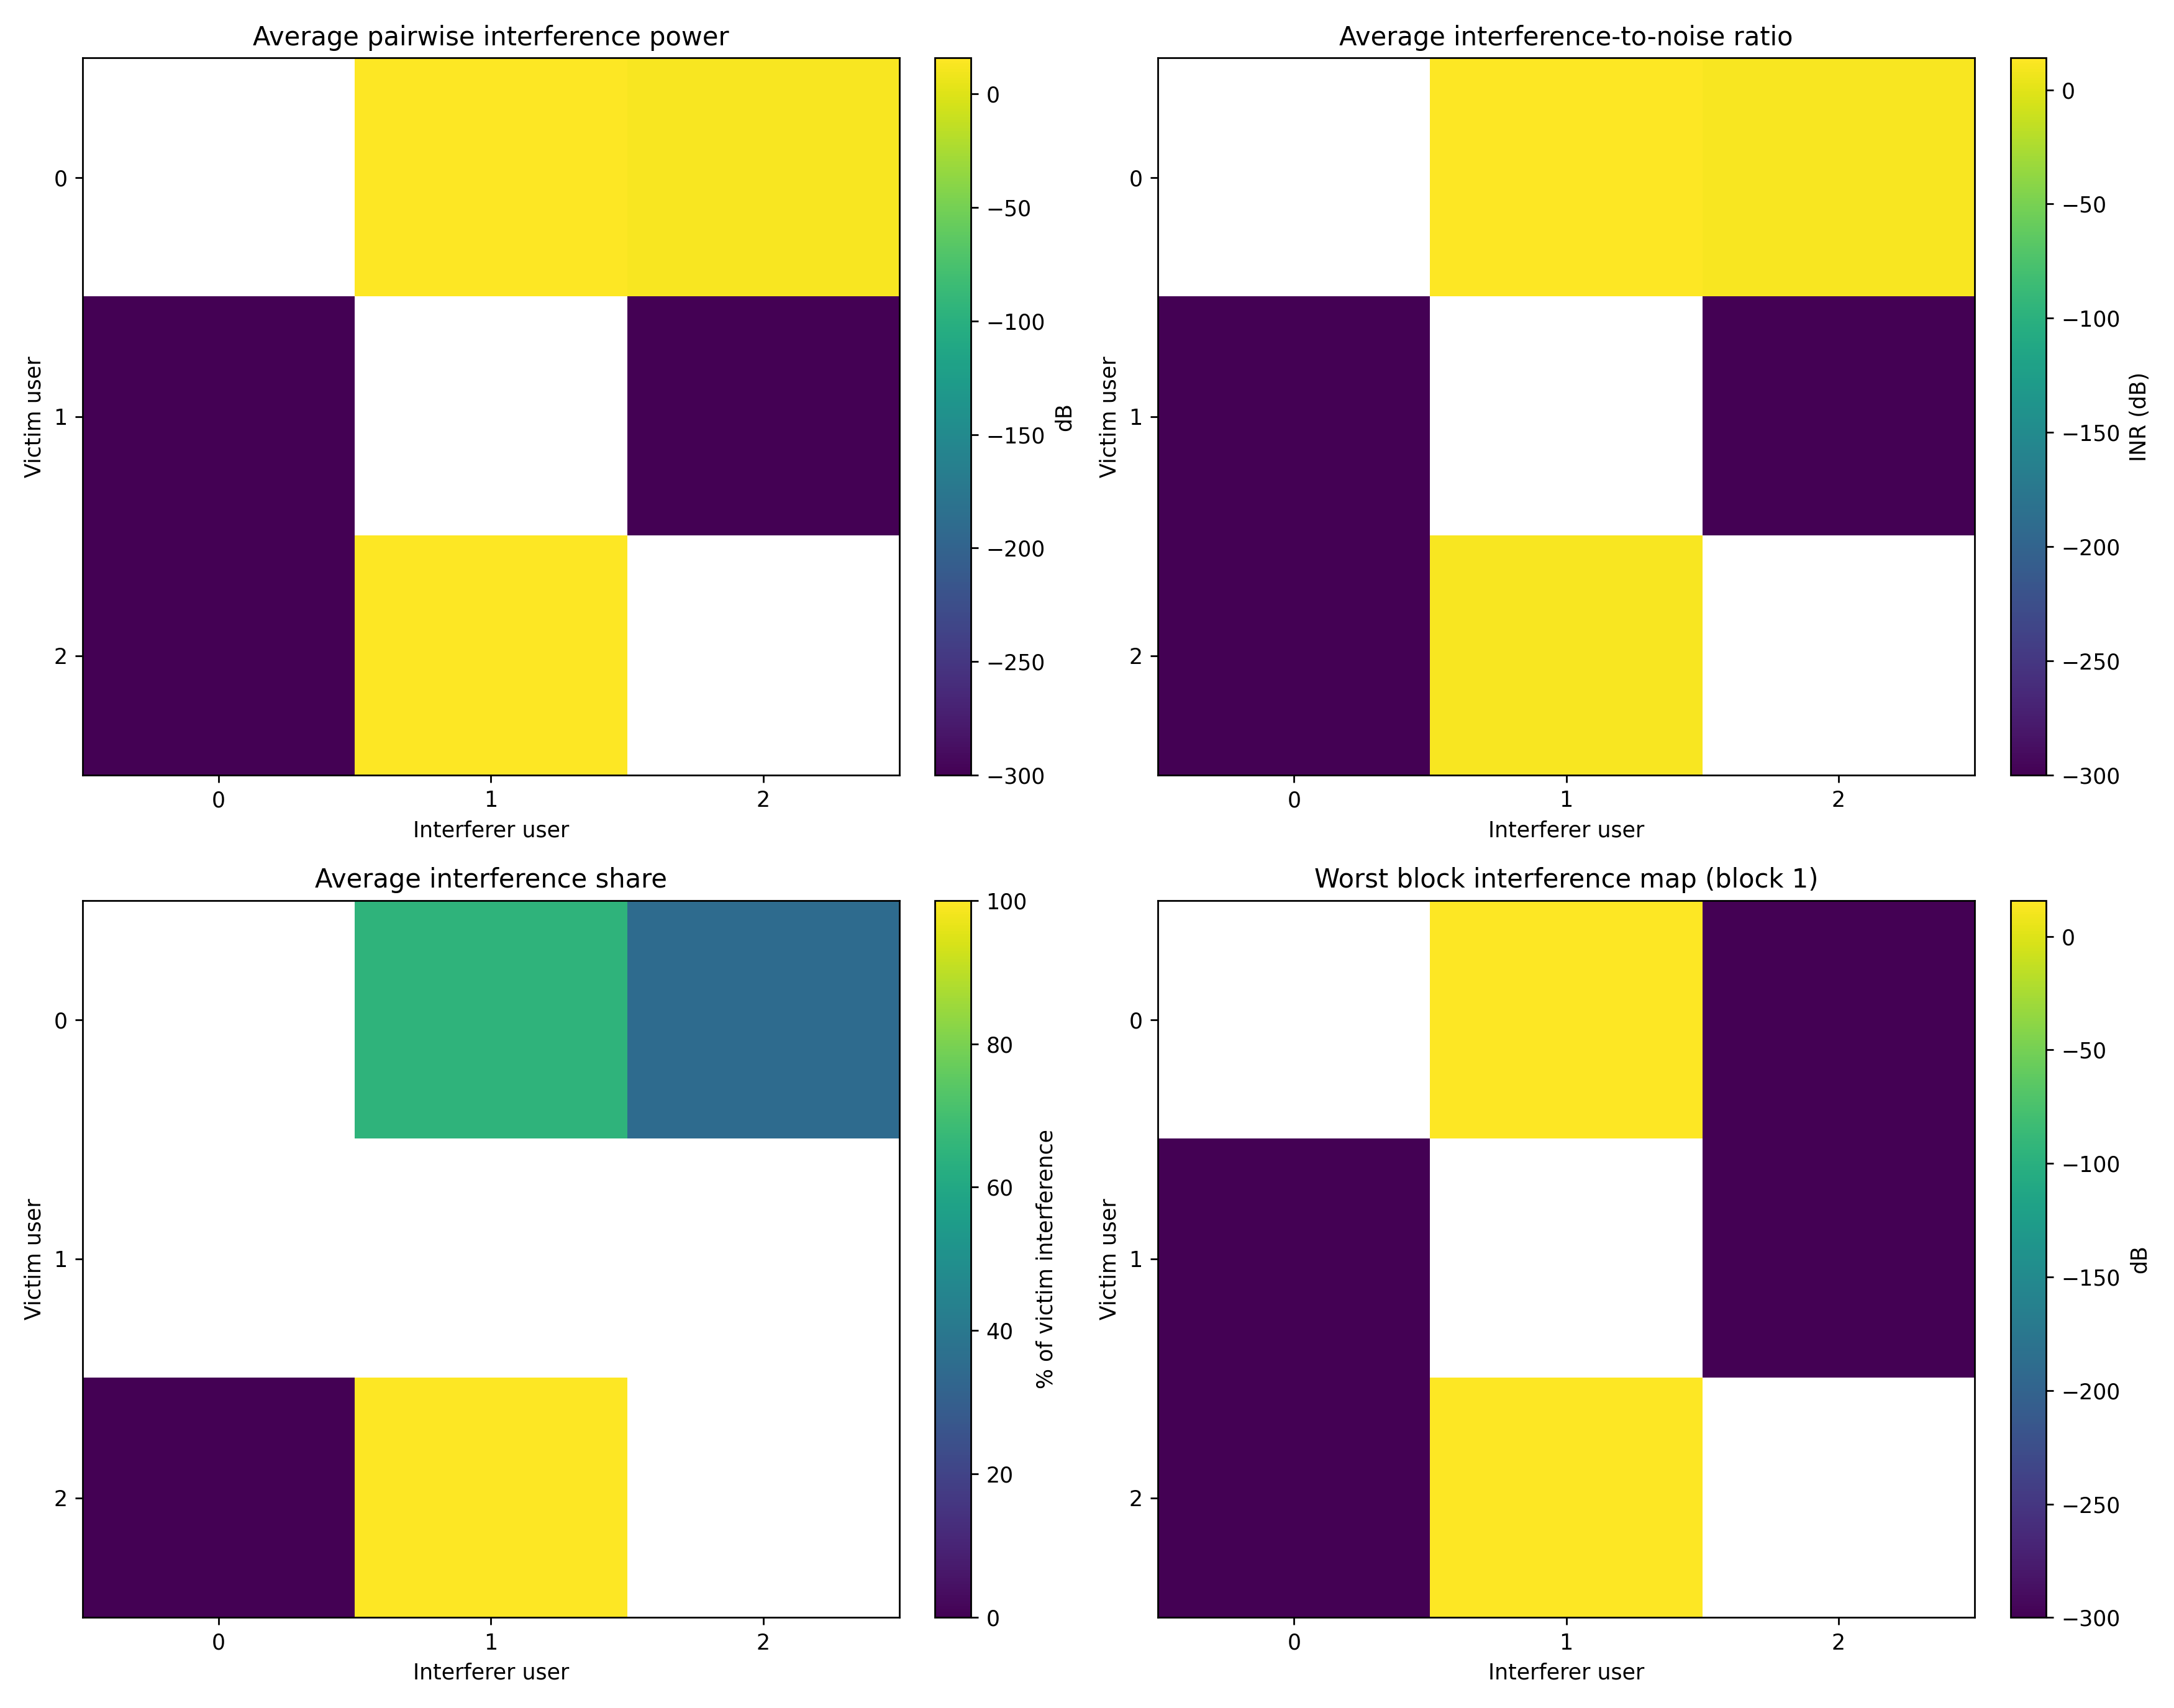
\includegraphics[width=\textwidth]{dl_payload_training_testing__interference_heatmaps.png}
    \caption{Training + Testing Method}
\end{subfigure}
\caption{Downlink payload-completion interference heatmaps.}
\end{figure}

\begin{figure}[H]
\centering
\begin{subfigure}[t]{0.48\textwidth}
    \centering
    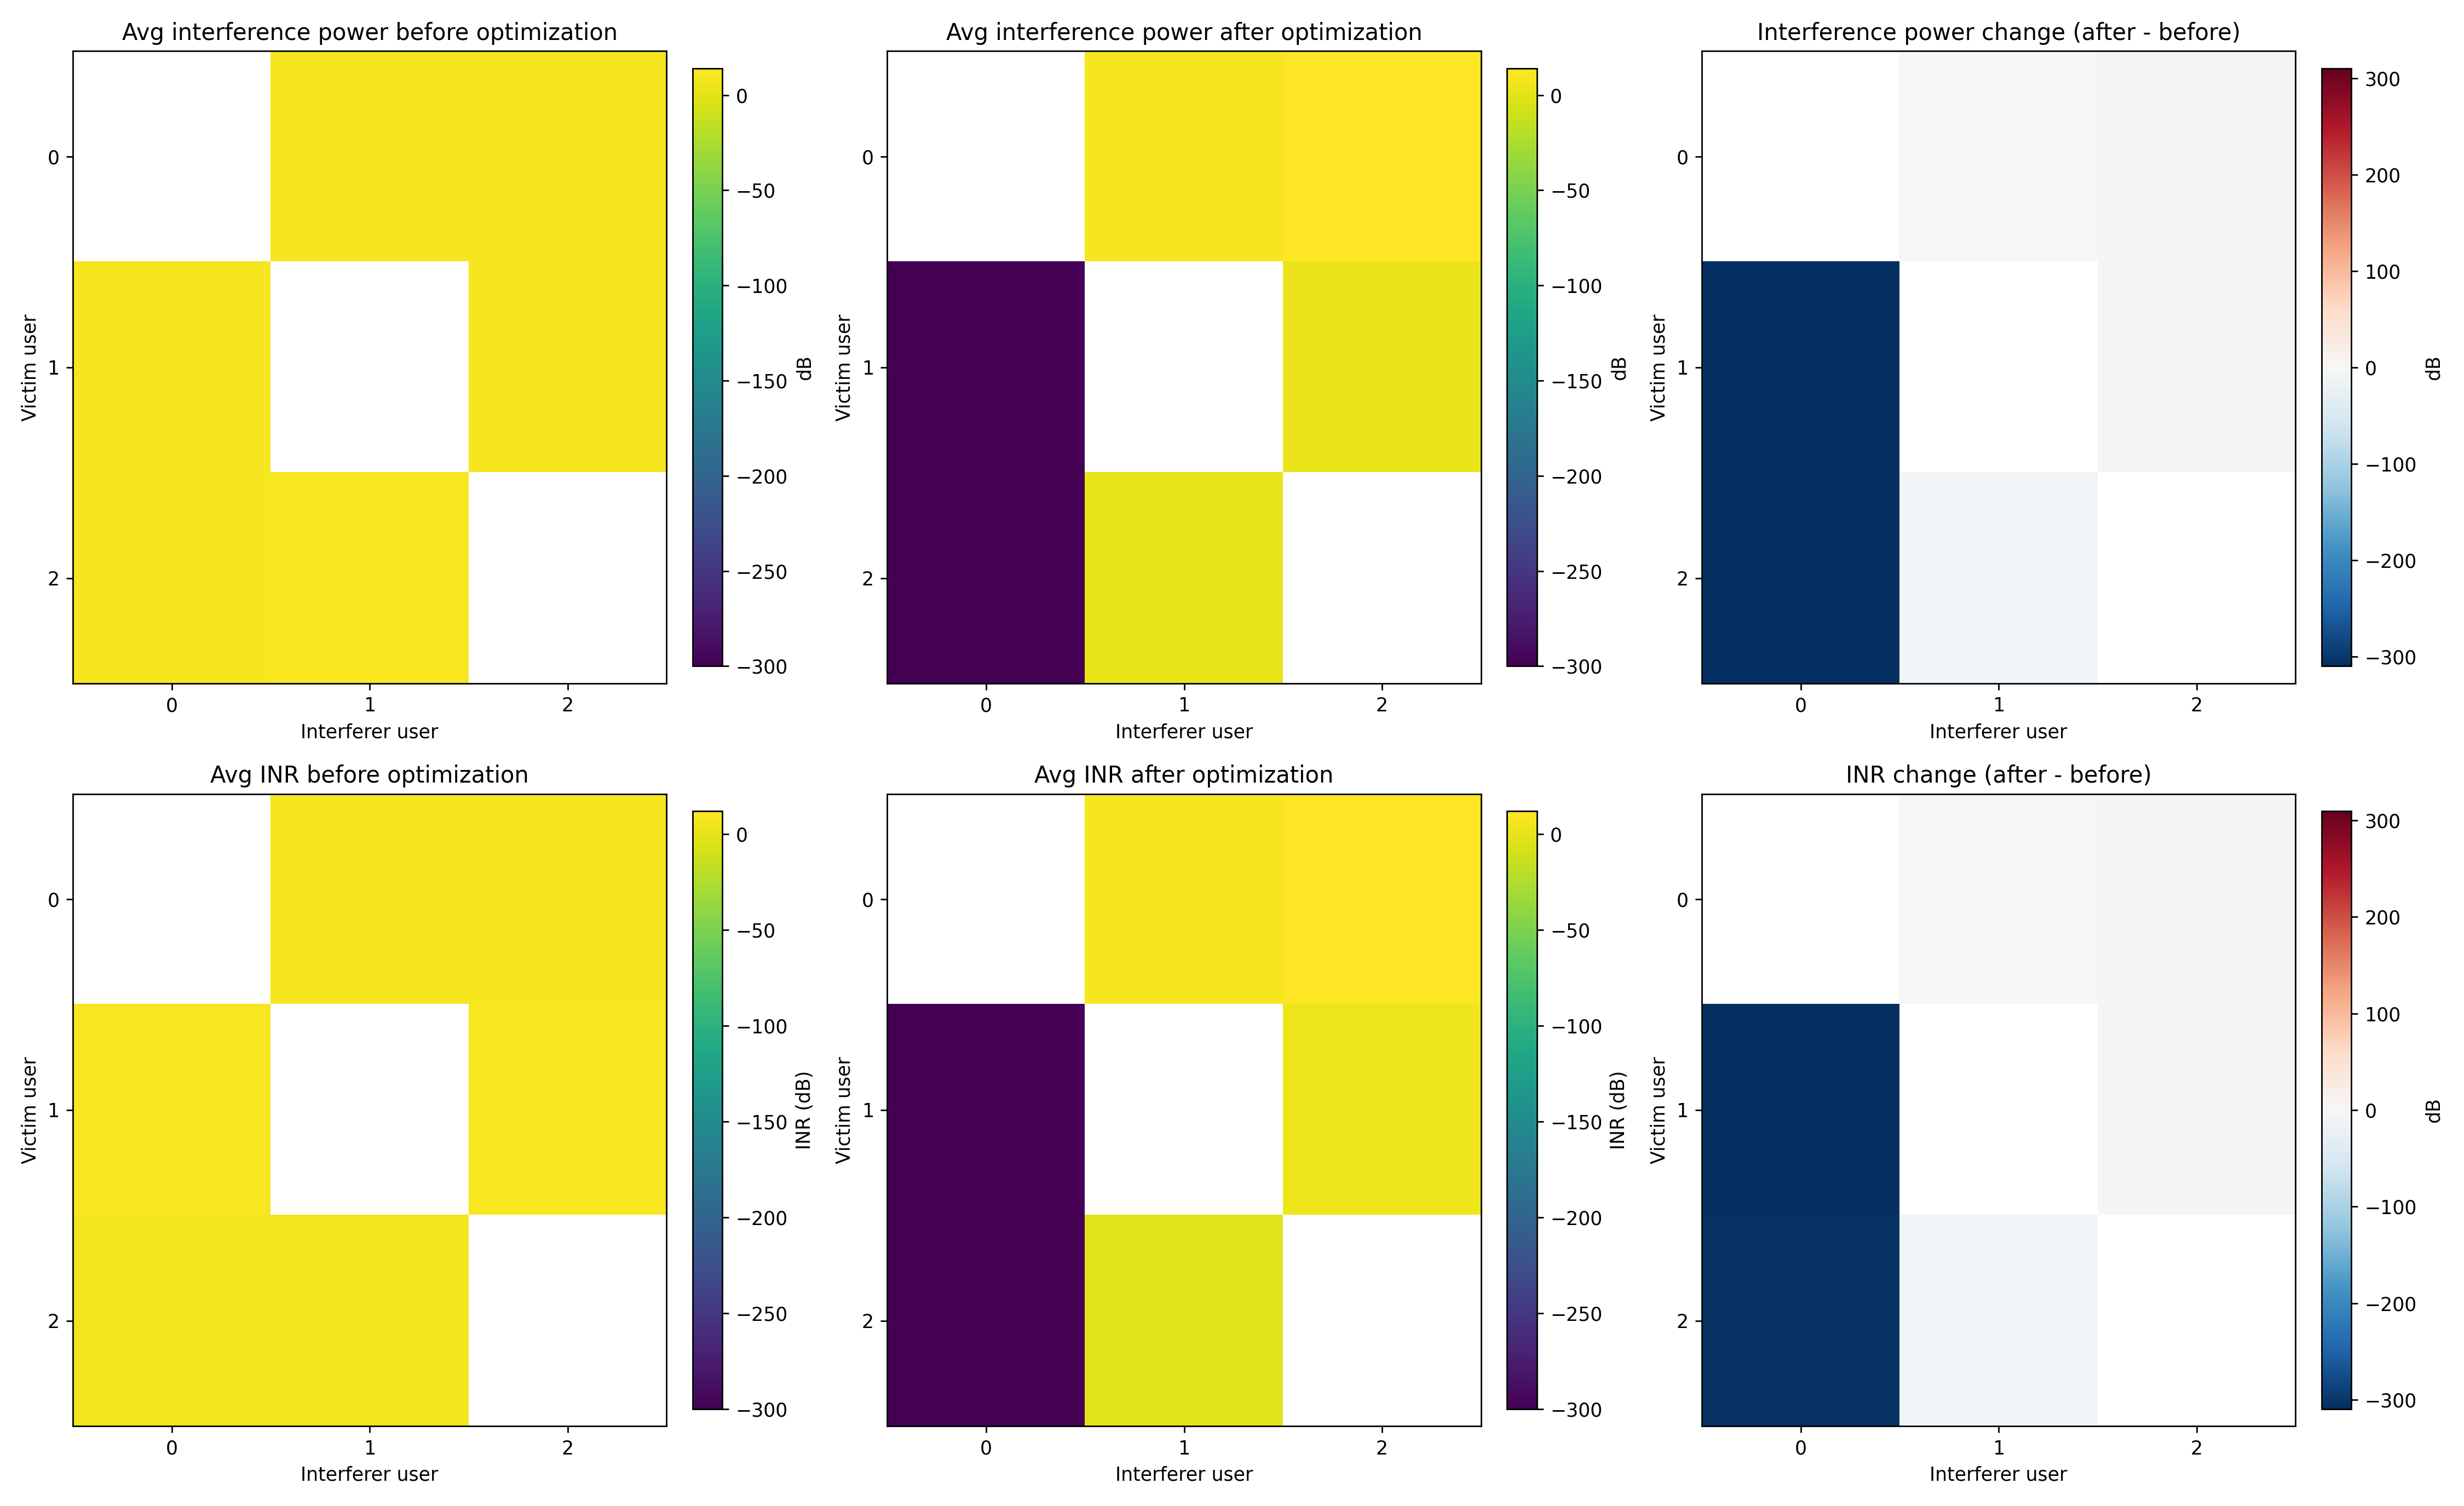
\includegraphics[width=\textwidth]{dl_payload_training_only__interference_before_after_heatmaps.png}
    \caption{Training Only Method}
\end{subfigure}
\hfill
\begin{subfigure}[t]{0.48\textwidth}
    \centering
    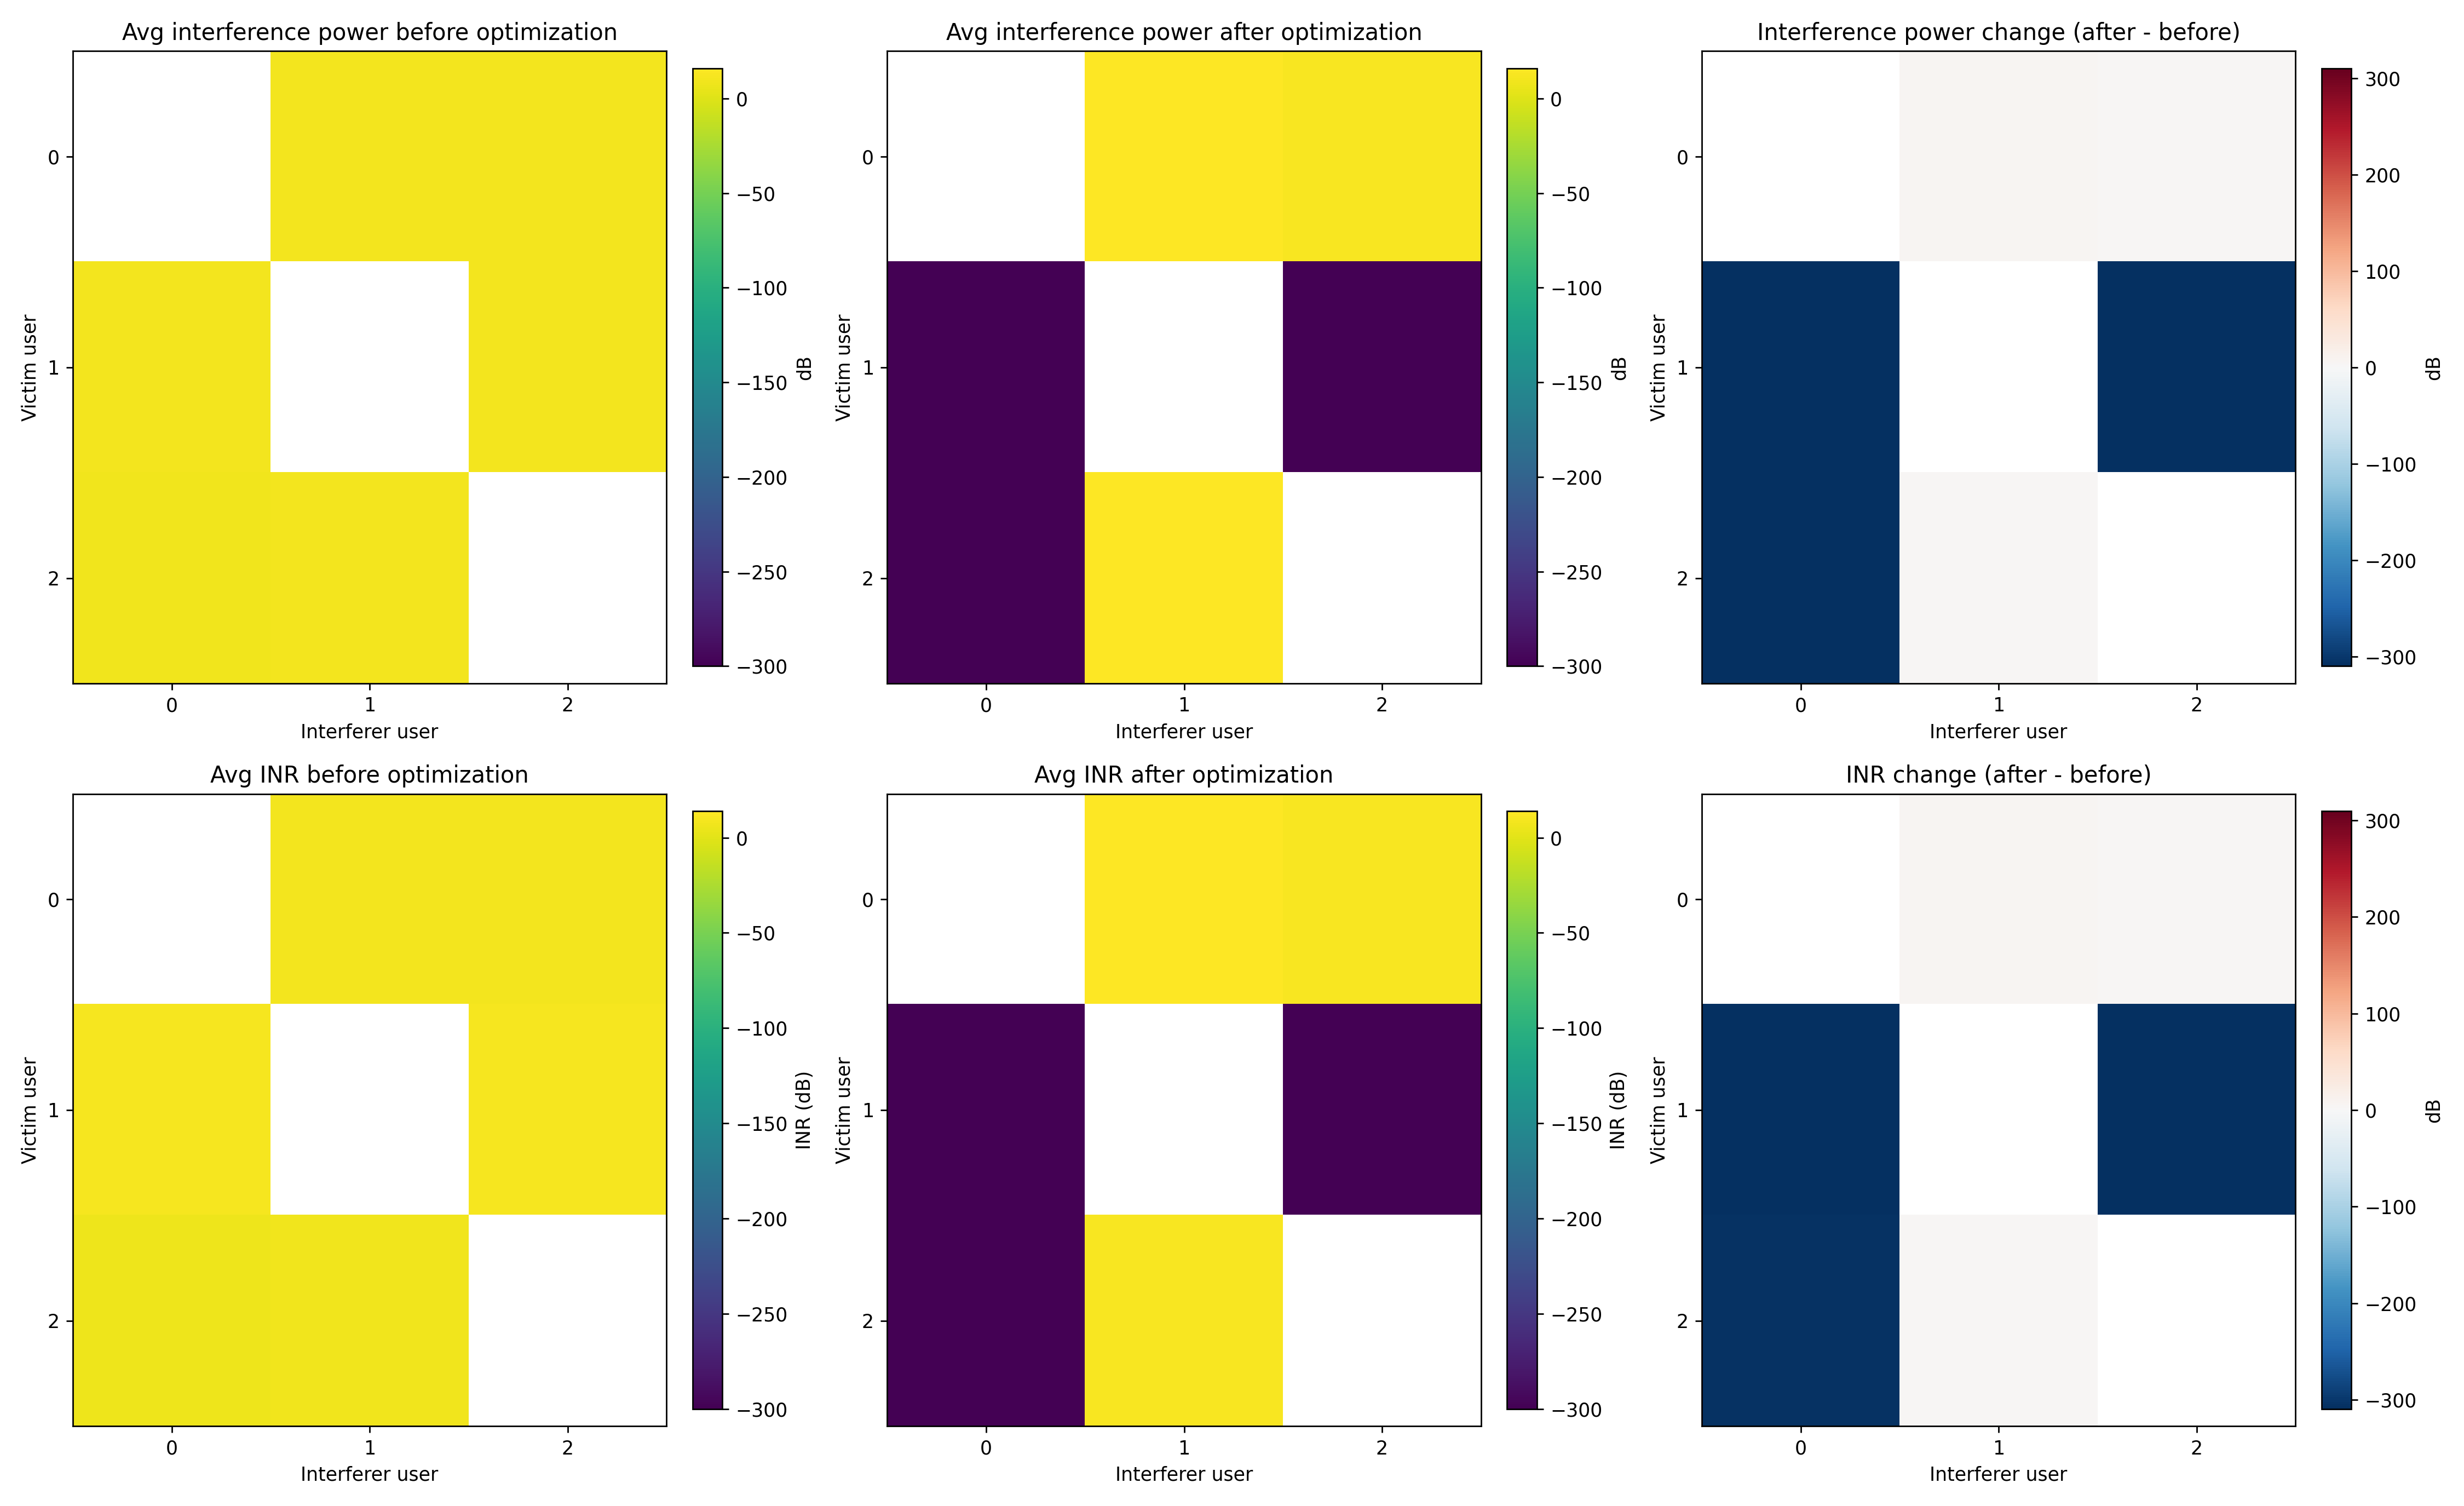
\includegraphics[width=\textwidth]{dl_payload_training_testing__interference_before_after_heatmaps.png}
    \caption{Training + Testing Method}
\end{subfigure}
\caption{Downlink payload-completion before/after heatmap comparison.}
\end{figure}

\section{Interference Takeaways}

Across all exported figures, the uplink remains the closer match between
methods. Its interference figures mostly show small SINR redistributions inside
a similar operating range. The downlink is more revealing. In payload
completion, the benchmark concentrates service more decisively on the currently
useful users.

\end{document}
